\documentclass[11pt]{article}
% Preamble for "How a Proof Becomes a Program" — the LaTeX-source edition.
% Compiles with pdflatex (pure-ASCII source; all math via LaTeX commands).

\usepackage[T1]{fontenc}
\usepackage{textcomp}
\usepackage{amsmath}
\usepackage{amsthm}
\usepackage{mathtools}
\usepackage{newpxtext}                 % Palatino-family text (book-quality serif)
\usepackage{newpxmath}                 % matching math (provides \mathbb, etc.)
\usepackage[varqu,scaled=0.94]{zi4}    % Inconsolata monospace
\usepackage{microtype}

\usepackage[letterpaper,margin=1.15in]{geometry}
\usepackage{xcolor}
\usepackage{booktabs}
\usepackage{array}
\usepackage{enumitem}
\setlist{itemsep=3pt,topsep=5pt,parsep=0pt}

\usepackage{titlesec}
\titleformat{\section}{\normalfont\Large\bfseries\color{accent}}{}{0pt}{}
\titleformat{\subsection}{\normalfont\large\bfseries}{}{0pt}{}
\titlespacing*{\section}{0pt}{1.9\baselineskip}{0.8\baselineskip}
\titlespacing*{\subsection}{0pt}{1.2\baselineskip}{0.4\baselineskip}

\usepackage{tikz}
\usetikzlibrary{arrows.meta,positioning,calc,fit,backgrounds,chains,
  shapes.geometric,shapes.misc,decorations.pathreplacing}
\usepackage{caption}
\captionsetup{font=small,labelfont={bf,color=accent},skip=6pt}

\usepackage[numbers,sort&compress]{natbib}
\usepackage[hidelinks]{hyperref}

% ---------- palette ----------
\definecolor{accent}{HTML}{1A5276}   % deep blue  (structure)
\definecolor{amber}{HTML}{B9770E}    % amber      (the "live" value)
\definecolor{good}{HTML}{1E8449}     % green      (choice-free / runs)
\definecolor{bad}{HTML}{922B21}      % red        (classical / does not run)
\definecolor{boxbg}{HTML}{F3F6F8}
\definecolor{boxbg2}{HTML}{FBF5EA}
\definecolor{rulec}{HTML}{9FB0BA}

% ---------- notation (\ensuremath so each works in text and math) ----------
\newcommand{\Nat}{\ensuremath{\mathbb{N}}}
\newcommand{\PT}{\mathsf{PureType}}          % math-only (subscripted)
\newcommand{\good}{\ensuremath{\operatorname{good}}}
\newcommand{\fib}{\ensuremath{\operatorname{fib}}}
\newcommand{\hydra}{\ensuremath{\operatorname{hydra}}}
\newcommand{\lev}{\ell}                       % math-only
\newcommand{\rz}{\ensuremath{\Vdash}}
\newcommand{\extract}{\ensuremath{\mathsf{extract}}}
\newcommand{\CtQ}{\ensuremath{\mathsf{CtQ}}}
\newcommand{\epsz}{\ensuremath{\varepsilon_0}}
\newcommand{\fst}{\pi_1}                       % math-only
\newcommand{\snd}{\pi_2}                       % math-only
\newcommand{\code}[1]{\texttt{#1}}

% a key statement, set off as an indented italic callout with an accent rule
\newenvironment{keystmt}{%
  \par\smallskip\noindent\begin{list}{}{%
    \setlength{\leftmargin}{1.6em}\setlength{\rightmargin}{1.2em}%
    \setlength{\topsep}{4pt}}\item[\textcolor{accent}{\rule[-0.2ex]{2.2pt}{1.2em}}]\itshape}%
  {\end{list}\smallskip}

% ---------- tikz styles ----------
\tikzset{
  box/.style={draw=accent,line width=0.7pt,rounded corners=2.5pt,fill=boxbg,
    inner sep=6pt,align=center,font=\small,minimum height=2.4em},
  boxa/.style={box,draw=amber,fill=boxbg2},
  boxg/.style={box,draw=good,fill=good!8},
  boxb/.style={box,draw=bad,fill=bad!7},
  plain/.style={inner sep=3pt,align=center,font=\small},
  flow/.style={-{Latex[length=2.4mm,width=1.8mm]},line width=0.8pt,draw=accent!85!black},
  flowa/.style={flow,draw=amber!85!black},
  ladder/.style={draw=rulec,line width=0.6pt,-{Latex[length=2mm]}},
  elabel/.style={font=\footnotesize\itshape,fill=white,inner sep=1.5pt,text=black!70},
  figcap/.style={font=\footnotesize,text=black!65,align=center},
  % --- descent-certificate motif (repeated across Act IV) ---
  dbox/.style={draw=accent,line width=0.6pt,rounded corners=2pt,fill=boxbg,
    inner sep=0pt,minimum width=8mm,minimum height=6.5mm,font=\footnotesize,align=center},
  dzero/.style={dbox,draw=good,fill=good!12},          % the certificate hits bottom
  dup/.style={dbox,draw=amber,fill=boxbg2},            % the visible quantity, climbing
  dlab/.style={font=\footnotesize\itshape,text=accent},% "descent certificate: ..."
}


\title{\bfseries How a Proof Becomes a Program\\[6pt]
  \normalfont\large\itshape A visual tour of a small formal system in which
  theorems, once proved, hand you a working program\\ --- and of what that
  turns out to cost.}
\author{Ara Aslyan}
\date{}

\begin{document}
\maketitle
\thispagestyle{empty}

%======================================================================
\section*{Prologue}

In school we learn that a proof is something that convinces us a statement
is true. A proof of ``every even number greater than two is a sum of two
primes'' would settle the matter; it would not, on the face of it, \emph{do}
anything.

Computer scientists discovered something stronger. Sometimes a proof does
not merely establish that an object exists --- it contains, inside itself, a
recipe for \emph{building} that object. A proof that ``every list can be
sorted'' can hide an actual sorting algorithm in its steps. When that
happens, the proof is not just an argument; it is a program in disguise, and
with the right lens you can read the program straight off the proof. Proof
assistants --- software that checks proofs down to the last symbol --- let us
apply that lens \emph{mechanically}, turning a verified proof into runnable
code with no human cleverness in between.\footnote{The development this tour
describes is carried out in Lean~4~\citep{demoura2021} with its mathematical
library Mathlib~\citep{mathlib2020}; the extensional-collapse layer it builds
on is a companion Kleene--Kreisel continuous-functionals development.
Throughout, ``the proof assistant'' and ``the machine'' mean this system.}

For simple statements this is unsurprising. The interesting question is what
happens at the other extreme. Some theorems need reasoning far stronger than
ordinary arithmetic --- reasoning that climbs past the natural numbers into
the infinite, using principles a first course in induction never mentions.
When a proof reaches that high, does the program still fall out the bottom?
Or does the extra strength leave a residue --- some step that asserts an
object exists without ever building it --- that quietly hollows the extracted
program into something that type-checks but cannot actually run?

This document answers that question by opening one such extraction pipeline
from end to end. We take a fixed, small formal system; we prove inside it a
theorem that genuinely needs more than ordinary induction; we watch, in full
detail, the proof become a program; and we then ask the proof assistant,
which cannot lie, exactly which assumptions that program depends on. The
tour is meant to be read start to finish by someone who has never seen any
of this before. Everything is built up on the page, and each idea arrives at
the moment an earlier paragraph has made you ask for it.

%======================================================================
\section{Act I --- The hook}

Pick a natural number --- say $3$. Write it down. Now play the following
game with it.

First, rewrite the number using only powers of $2$, and rewrite the
exponents that way too, and their exponents, all the way down, until nothing
but $2$s and small constants remain. This is called \emph{hereditary base
$2$}. Now change every $2$ you wrote into a $3$ --- bump the base --- and
subtract $1$ from the result. Then rewrite \emph{that} number in hereditary
base $3$, change every $3$ into a $4$, subtract $1$ again. Then base $4$ into
base $5$, subtract $1$. And so on, bumping the base by one each step and
subtracting a single unit each time.

The bases are marching upward without bound. Each step replaces a base by a
larger one everywhere it appears --- and near the start, that base change
inflates the number far more violently than the lonely ``subtract $1$'' ever
pulls it back down. The sequence you are generating does not drift gently;
for many starting values it erupts. Start at $4$ and the first terms are
those in Figure~\ref{fig:erupt}: the number climbs into values with no short
decimal name --- and yet, eventually, it comes back down to $0$.

\begin{figure}[h]
\centering
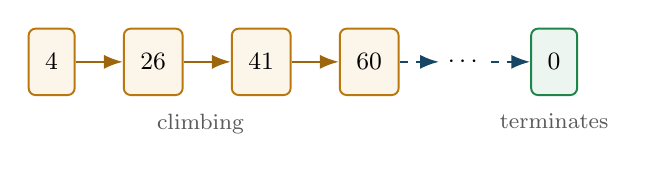
\begin{tikzpicture}[node distance=6mm]
  \node[boxa](n0){$4$};
  \node[boxa,right=of n0](n1){$26$};
  \node[boxa,right=of n1](n2){$41$};
  \node[boxa,right=of n2](n3){$60$};
  \node[plain,right=5mm of n3](d){$\cdots$};
  \node[boxg,right=5mm of d](z){$0$};
  \draw[flowa](n0)--(n1); \draw[flowa](n1)--(n2); \draw[flowa](n2)--(n3);
  \draw[flow,dashed](n3)--(d); \draw[flow,dashed](d)--(z);
  \node[figcap,below=1mm of n1,xshift=6mm]{climbing};
  \node[figcap,below=1mm of z]{terminates};
\end{tikzpicture}
\caption{The Goodstein sequence starting at $4$: it erupts upward, driven by
the base change, then --- after astronomically many steps --- reaches
exactly $0$. (The sequence starting at $3$ is tame by comparison:
$3,3,3,2,1,0$.)}
\label{fig:erupt}
\end{figure}

Goodstein's theorem~\citep{goodstein1944} says that this sequence --- no matter
which number you started from --- always, eventually, hits exactly $0$.

That is already strange. A process whose every early move makes the number
enormously bigger, driven downward only by subtracting one at a time,
nonetheless terminates at $0$ for \emph{every} starting value. But the
strange part, for our purposes, is not the theorem itself. It is what it
takes to prove it, and what you can do with the proof once you have it.

Here is the first half of the surprise. You cannot prove Goodstein's theorem
with ordinary mathematical induction over the natural numbers. The usual
``check $0$, then check that each number's truth follows from the previous
one'' is genuinely not enough; the theorem needs a stronger principle, one
that reaches past where step-by-step induction on $\Nat$ can go. (Exactly
what that stronger principle is, and why it is stronger, is Act~IV's
business. For now, hold onto the fact that ordinary induction falls short.)

Here is the second half. Despite needing that extra strength, the proof is
\emph{constructive} --- it does not merely assert that the sequence reaches
$0$, it contains, buried inside it, a recipe for finding the exact step at
which that happens. And in the formal system this tour is about, that recipe
can be pulled out of the proof mechanically and run as an actual program.
Feed it a starting number; it returns the stopping step.

Most expositions of Goodstein's theorem stop at the statement, or gesture at
the proof and leave the ``constructive content'' as a phrase. This one opens
the box all the way. We are going to watch, in complete detail and on a real
example, a proof turn into a program --- first on something tiny enough to
hold in your hand, then on Goodstein itself, and then on a handful of other
theorems that each ask the machine to do one genuinely new thing. By the end
you will have seen the whole mechanism, and one question will remain: when a
program falls out of a proof this powerful, does some sliver of
non-constructive reasoning sneak into the program along the way? The last act
is devoted to answering it.

%======================================================================
\section{Act II --- One tiny, real example, walked through completely}

Before any general theory, one concrete thing, done slowly and in full. We
will not introduce a single piece of machinery in this act beyond what this
one example forces us to name. No hierarchies, no levels, no collapses ---
those are Act~III, and they will make far more sense once you have a real
realizer in hand to point at.

Everything in this tour happens inside a fixed, small formal system --- we
will call it \emph{the fragment}. Think of the fragment as a self-contained
little world of mathematics with a rigid rulebook: a fixed vocabulary of
things it can talk about (zero, successor, addition, multiplication, and a
modest list of further operations we meet as we need them), a fixed grammar
of statements it can form, and a fixed list of inference rules for building
proofs. Nothing enters the fragment except through that rulebook. This
rigidity is deliberate: because the rules are finite and mechanical, a proof
in the fragment is itself a finite, mechanical object --- a tree of
rule-applications --- and a machine can take that tree apart. Hold that
thought; it is what makes everything later possible.

Our example is the fragment's very first existential theorem --- the first
time it proved that \emph{something exists} rather than that two things are
equal. It is deliberately the warm-up the development itself used before
tackling the general Goodstein theorem, and we use it for exactly that
reason: in Act~IV, Goodstein will be the grown-up version of this same
statement, and you will already have watched the miniature happen by hand.
The statement is: \emph{there is a step $s$ at which the Goodstein sequence
starting from $3$ has reached $0$}, written in the fragment's grammar as
\[
  \exists s.\ \good(3,s)=0,
\]
where $\good(3,s)$ is the fragment's own name for ``the value of the
Goodstein sequence started at $3$, after $s$ steps.''

We happen to know the answer. The Goodstein sequence starting from $3$ runs
$3,3,3,2,1,0$, so it first reaches $0$ at step~$5$. The number~$5$ is the
\emph{witness}: the particular $s$ that makes $\exists s.\ \good(3,s)=0$
true. Keep~$5$ in mind; the whole act is about watching it travel from the
proof into a running program and back out.

\subsection*{What a realizer for this has to be}

Here is the first idea we genuinely need, and it arrives because the
statement forces it. The statement claims something \emph{exists}. A proof
that merely convinces us the claim is true --- without ever saying
\emph{which} $s$ works --- would be useless for computing anything. So we
ask: what would a proof have to carry, concretely, for us to read the answer
off it?

At a minimum, it has to carry the witness --- the number $5$ --- because
without it there is nothing to return. And it has to carry, as well, some
evidence that this witness really does the job: that $\good(3,5)$ really is
$0$. This ``what a proof carries'' is exactly the notion of a
\textbf{realizer}: the computational content of a proof, the data a machine
can actually use. The shape of that data is dictated by the statement's
outermost connective, and for an existential it is precisely the pair we
just argued for:
\begin{keystmt}
A realizer of $\exists y.\ \varphi(y)$ is a pair $x$: a \textbf{witness}
$\fst x$, and a \textbf{certificate} $\snd x$ that realizes $\varphi$ at that
witness. Compactly,
\[
  x \rz \exists y.\ \varphi(y)
  \quad\Longleftrightarrow\quad
  \snd x \rz \varphi\bigl(\fst x\bigr).
\]
\end{keystmt}
Read $\fst x$ as ``read the witness off $x$'' and $\snd x$ as ``the rest of
$x$.'' This is not a metaphor chosen for this paper; it is the actual clause
the fragment uses to define what ``realizes'' means at an existential.

Now specialize it to our formula. Instantiating the clause at
$\exists s.\ \good(3,s)=0$ gives
\[
  x \rz \exists s.\ \good(3,s)=0
  \quad\Longleftrightarrow\quad
  \snd x \rz \bigl(\good(3,\fst x)=0\bigr).
\]
The body $\good(3,s)=0$ is an \emph{equation}, and here a second small idea
appears, again forced by the example. What does it take to realize an
equation? An equation is either true or not; if it is true, there is nothing
further to \emph{compute} about it --- no witness to choose, no case to
decide. So the realizer of a true equation carries no information at all: any
object realizes it, provided the equation holds. We call such a realizer
\textbf{contentless}. So the certificate $\snd x$ above is contentless, and
the realizer of $\exists s.\ \good(3,s)=0$ is, in effect, \emph{just the
witness $5$} wearing a trivial second component. All of the content is the
witness. That is as simple as a realizer ever gets, which is why we started
here.

\subsection*{The proof, and what \texorpdfstring{$\extract$}{extract} does to it}

Now we build an actual proof of $\exists s.\ \good(3,s)=0$ in the fragment,
in the shape the realizer analysis predicts. To prove an existential the
fragment has a rule --- existential introduction --- that says: to conclude
$\exists y.\ \varphi$, supply a specific term for $y$ and a proof that
$\varphi$ holds for that term. We supply the term $5$. That leaves us needing
a fragment-internal proof that $\good(3,5)=0$ --- and this the fragment can
simply \emph{compute}, grinding its defining equations for $\good$ on the
concrete numbers $3$ and $5$ until it reaches $0$. So the whole proof is:
existential-introduction, at $5$, over the computed equation, a small tree
with the witness $5$ at the branch point.

The fragment comes with a function --- $\extract$ --- that takes a finished
proof and returns its realizer, by walking the proof tree and doing, at each
rule, the small operation that rule's realizer calls for. On our proof it
does exactly what the shape predicts (Figure~\ref{fig:extract2}): the witness
$5$ the rule supplied becomes the pair's first component; the realizer of the
computed equation --- contentless --- becomes the second. And to run the
result, we read its first component at the canonical point, recovering $5$.

\begin{figure}[h]
\centering
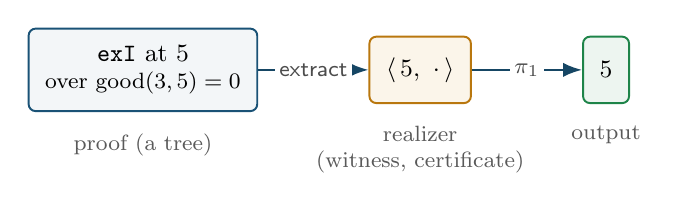
\begin{tikzpicture}[node distance=14mm]
  \node[box,align=center](p){\code{exI} at $5$\\[-1pt]\footnotesize over $\good(3,5)=0$};
  \node[boxa,right=of p](r){$\langle\,5,\ \cdot\,\rangle$};
  \node[boxg,right=of r](o){$5$};
  \draw[flow](p)--node[elabel]{$\extract$}(r);
  \draw[flow](r)--node[elabel]{$\fst$}(o);
  \node[figcap,below=1.5mm of p]{proof (a tree)};
  \node[figcap,below=1.5mm of r]{realizer\\(witness, certificate)};
  \node[figcap,below=1.5mm of o]{output};
\end{tikzpicture}
\caption{The whole round trip on the tiny example. The proof already
contains the witness $5$; $\extract$ only repackages it into the standard
existential shape $\langle\text{witness},\text{certificate}\rangle$, the
certificate contentless because the body is an equation. Reading the first
component returns $5$.}
\label{fig:extract2}
\end{figure}

That is the full round trip on the smallest possible real example: a
statement was formed; we reasoned out what a proof of it must carry; we built
such a proof by hand; $\extract$ repackaged its witness; evaluating the
result returned $5$. Nothing here required knowing what a ``level'' is, where
realizers ``live,'' or how any of this scales. Those questions push
themselves on us the moment we ask ``does this work for \emph{every} proof?''
--- and Act~III introduces exactly the machinery they demand.

%======================================================================
\section{Act III --- Opening the box}

We have watched one proof become one program. Two questions are now
unavoidable. First: our example's body was an equation, whose realizer was
contentless --- so \emph{this} realizer was essentially just a number. Real
theorems have bodies with ``and,'' ``or,'' implications, ``for all.'' What
are realizers of \emph{those}? Second: we ran $\extract$ once and got the
right answer. Is that luck, or does $\extract$ produce a correct realizer for
\emph{every} proof? We take the questions in that order, because the second
needs the first.

\subsection*{Realizers, for every shape of statement}

In Act~II we met the realizer clause for $\exists$ by asking what a proof of
an existential must carry. Every connective has such a clause, arrived at the
same way, and once you have seen one the rest are recognizable rather than
surprising.\footnote{The interpretation is Kreisel's \emph{modified}
realizability~\citep{kreisel1959}; the standard reference, whose
induction-axiom realizer this development follows, is
Troelstra~\citep{troelstra1973}.} Table~\ref{tab:realizers} collects them --- the guiding question
each time being \emph{what would a machine need to use a proof of this?}

\begin{table}[h]
\centering
\renewcommand{\arraystretch}{1.35}
\begin{tabular}{@{}l l l@{}}
\toprule
\textbf{Statement} & \textbf{Realizer} & \textbf{to use a proof of it, you\dots} \\
\midrule
$s = t$ & (nothing) & \dots{}need nothing --- it just has to hold \\
$A \land B$ & a pair $(r_A, r_B)$ & \dots{}get at each side \\
$A \lor B$ & a tag $+$ a payload & \dots{}first learn which side \\
$A \rightarrow B$ & a function $r_A \mapsto r_B$ & \dots{}feed it evidence of $A$ \\
$\forall x.\ A(x)$ & a function $k \mapsto r_{A(k)}$ & \dots{}pick an $x$ \\
$\exists x.\ A(x)$ & a pair (witness, certificate) & \dots{}read the witness \\
\bottomrule
\end{tabular}
\caption{What realizes each shape of statement. An equation is
\emph{contentless}. A conjunction holds both realizers at once; a disjunction
tags which side holds ($0$ left, non-zero right) and carries that side's
realizer --- structurally the same ``a number, then a payload it selects''
as the existential, which is why the fragment builds $\exists$ out of the
disjunction's pairing machinery. The two that \emph{consume} an input --- the
functions of $\rightarrow$ and $\forall$ --- are the ones that do work at
runtime.}
\label{tab:realizers}
\end{table}

You have now seen the shape of every realizer the fragment will ever produce.
Two of them --- implication and universal --- take something in and give
something back; they are the procedures, the parts that \emph{do work} at
runtime. To use a proof of ``if $A$ then $B$'' you feed it evidence of $A$
and it returns evidence of $B$; to use ``for all $x$'' you pick an $x$ and it
returns the instance. The other three --- pair, tag, witness --- just
\emph{hold} data. Keep that distinction in view; the next section --- levels
--- is built entirely on it.

\subsection*{Levels: the cost of consuming}

Here is the question the previous paragraph forced. Implications and
universals are procedures --- they take an input and return an output. But
that input is \emph{itself} a realizer, which might itself be a procedure
taking an input, and so on. A realizer can be a procedure whose inputs are
procedures whose inputs are procedures. How deep does the nesting go, and how
do we track it?

The fragment tracks it with a single number on each formula, its
\textbf{level} $\lev$, counting how many layers of ``takes an input, returns
an output'' a realizer can involve. The counting rule is short, and it is
exactly the consume-versus-hold distinction made arithmetic:
\begin{align*}
  \lev(s=t)              &= 0, &
  \lev(A \rightarrow B)  &= \max\bigl(\lev A + 1,\ \lev B\bigr), \\
  \lev(A \land B)        &= \max\bigl(\lev A,\lev B\bigr), &
  \lev(\forall x.\,A)    &= \lev A + 1, \\
  \lev(A \lor B)         &= \max\bigl(\lev A,\lev B\bigr), &
  \lev(\exists x.\,A)    &= \lev A.
\end{align*}
Only the two consuming connectives add a level. Why does $\forall$ cost a
level but $\exists$ does not, when both mention a bound variable? Because
$\forall y.\,\varphi$ is a \emph{procedure} --- you hand it a $y$ and it works
--- while $\exists y.\,\varphi$ merely \emph{holds} a $y$, the witness,
already chosen. A universal consumes; an existential packages. Consuming
costs a level; packaging is free. Look back at Act~II: the witness $5$ was
already sitting in the realizer, waiting to be read; nothing had to be
\emph{run}. That is exactly why our existential example was so simple:
$\exists$ adds no level. The rule is not imposed from outside --- it falls
straight out of the difference between a realizer that runs and one that
merely stores.

\subsection*{Where a realizer lives: \texorpdfstring{$\PT$}{PureType}}

We keep saying a realizer ``is a number,'' or ``is a procedure taking a
realizer and returning a realizer.'' Once realizers can be procedures whose
inputs are procedures, we must say precisely what mathematical objects these
are. Now that Act~II has given us a concrete realizer, and levels have told
us how deep the nesting goes, we can place them. Realizers live in a tower of
types, built by that same level count:
\[
  \PT_0 = \Nat, \qquad
  \PT_{n+1} = \bigl(\PT_n \to \Nat\bigr).
\]
The bottom floor is the natural numbers --- where a bare witness like our $5$
lives. Each floor up is the functions from the floor below to the numbers
(Figure~\ref{fig:tower}). Each time a formula's level rises by one --- each
time you add an implication or universal that \emph{consumes} a realizer ---
the realizer climbs one storey: a realizer of a level-$n$ formula lives $n$
storeys up. This is why we spent so long on levels first: the level is the
floor number.

\begin{figure}[h]
\centering
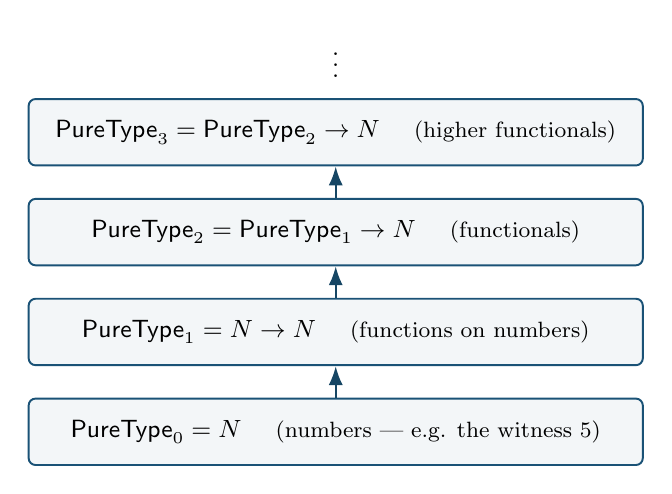
\begin{tikzpicture}[node distance=4mm]
  \node[box,minimum width=78mm](l0){$\PT_0=\Nat$ \quad\footnotesize (numbers --- e.g. the witness $5$)};
  \node[box,minimum width=78mm,above=of l0](l1){$\PT_1=\Nat\to\Nat$ \quad\footnotesize (functions on numbers)};
  \node[box,minimum width=78mm,above=of l1](l2){$\PT_2=\PT_1\to\Nat$ \quad\footnotesize (functionals)};
  \node[box,minimum width=78mm,above=of l2](l3){$\PT_3=\PT_2\to\Nat$ \quad\footnotesize (higher functionals)};
  \node[plain,above=1.5mm of l3](d){$\vdots$};
  \draw[flow](l0)--(l1); \draw[flow](l1)--(l2); \draw[flow](l2)--(l3);
\end{tikzpicture}
\caption{The $\PT$ tower. A realizer of a level-$n$ formula lives on floor
$n$. Our Act~II realizer was a level-$0$ object --- a number --- because its
formula, an existential over an equation, adds no level. This tower is built
by completely elementary means, with nothing classical or non-constructive
anywhere in it --- a fact Act~V will turn on.}
\label{fig:tower}
\end{figure}

\subsection*{The program a closed statement denotes: \texorpdfstring{$\CtQ$}{CtQ}}

Two \emph{different} proofs of the same statement can produce two different
realizers --- different objects in the tower --- that nonetheless compute the
same answers everywhere. To speak of ``\emph{the} program'' a theorem
denotes, we collapse realizers that agree as functions into single objects.
For a closed statement, its realizer lands, after this collapse, in a space
the development calls $\CtQ$, and its image there is the one
\emph{proof-independent} program the theorem denotes:
\[
  \boxed{\ \text{Realizer}\ } \ \xrightarrow{\ \text{collapse}\ }\
  \boxed{\ \CtQ\ } .
\]
We name $\CtQ$ now but do not yet lean on it: for the collapse to be the
honest space of functionals rather than an arbitrary quotient, the realizers
landing in it must be \emph{continuous}, a property we state below. Read
$\CtQ$ for now as a promissory note --- \emph{the program of a closed theorem
is a single proof-independent object, once we know its realizer is
continuous} --- redeemed two definitions on.\footnote{$\CtQ$ is the
extensional collapse of the Kleene--Kreisel continuous
functionals~\citep{kleene1959,kreisel1959}; for a modern account see Longley
and Normann~\citep{longleynormann2015}.}

\subsection*{Soundness: it works for every proof}

Now the second opening question. We ran $\extract$ once and got a correct
realizer. Is that always so? It is --- and it is the central theorem of the
whole construction:
\begin{keystmt}
\textbf{Soundness.} For every proof the fragment can build, of every
statement, $\extract$ returns a genuine realizer of that statement.
\end{keystmt}
What we watched happen once, by hand, for $\exists s.\ \good(3,s)=0$,
soundness guarantees for \emph{every} derivation the fragment admits. Its
proof is itself an induction --- not over numbers, but over the shape of
proofs. There are finitely many inference rules; soundness checks, once, that
each rule's piece of $\extract$ does the right thing \emph{assuming the
pieces for its sub-proofs did}. Because every proof is a finite tree of those
rules, checking each rule once covers every proof there will ever be. From
here on we may speak of ``the program a theorem extracts to'' and know,
without further checking, that it is correct at every input.

\subsection*{Generic continuity: every program is continuous}

One more property, stated now and explained more deeply once Act~IV gives us
programs worth explaining it for. A realizer high in the tower is a
functional --- it takes functions as inputs. The pathological ones read
\emph{infinitely much} of their input before deciding an output, and those
are exactly the objects that do not collapse honestly into $\CtQ$. The good
functionals are the \textbf{continuous} ones: to determine any single output
they consult only \emph{finitely much} of their input. The development proves,
once and generically:
\begin{keystmt}
\textbf{Generic continuity.} Every realizer $\extract$ produces, from every
proof, is continuous.
\end{keystmt}
This redeems the promissory note on $\CtQ$: because every extract is
continuous, every closed theorem's realizer collapses honestly into a single
$\CtQ$ element --- one honest program. We will see \emph{why} generic
continuity holds in Act~VI; the harder examples of Act~IV should exist first
to make that ``why'' worth the space. The box is open: we have realizers for
every shape, the level accounting, the tower they live in, the collapse into
programs, and the two guarantees --- correctness and continuity. Everything
from here runs on exactly this machinery, unchanged. What varies is only the
proofs we feed it.

%======================================================================
\section{Act IV --- Running the same machine on harder proofs}

Nothing new gets added to the extractor in this act. The pipeline --- prove a
theorem, run $\extract$, get a certified program --- is fixed. What changes is
the difficulty of the proofs, and each example is chosen because it forces
exactly one genuinely new capability out of the same fixed machine. We name
that capability in a heading, so the staircase is visible
(Figure~\ref{fig:stair}). Before the first step, one rule the first five
examples all lean on.

\begin{figure}[h]
\centering
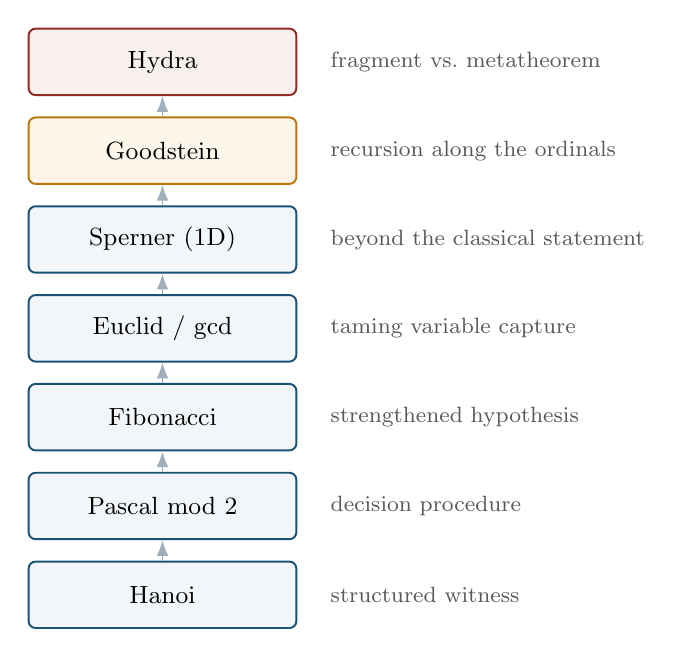
\begin{tikzpicture}[node distance=2.6mm]
  \node[box,minimum width=34mm](e1){Hanoi};
  \node[box,minimum width=34mm,above=of e1](e2){Pascal mod $2$};
  \node[box,minimum width=34mm,above=of e2](e3){Fibonacci};
  \node[box,minimum width=34mm,above=of e3](e4){Euclid / gcd};
  \node[box,minimum width=34mm,above=of e4](e5){Sperner (1D)};
  \node[boxa,minimum width=34mm,above=of e5](e6){Goodstein};
  \node[boxb,minimum width=34mm,above=of e6](e7){Hydra};
  \foreach \a/\b in {e1/e2,e2/e3,e3/e4,e4/e5,e5/e6,e6/e7}
    \draw[ladder](\a)--(\b);
  \node[figcap,right=3mm of e1,align=left]{structured witness};
  \node[figcap,right=3mm of e2,align=left]{decision procedure};
  \node[figcap,right=3mm of e3,align=left]{strengthened hypothesis};
  \node[figcap,right=3mm of e4,align=left]{taming variable capture};
  \node[figcap,right=3mm of e5,align=left]{beyond the classical statement};
  \node[figcap,right=3mm of e6,align=left]{recursion along the ordinals};
  \node[figcap,right=3mm of e7,align=left]{fragment vs.\ metatheorem};
\end{tikzpicture}
\caption{The staircase of Act~IV: each example is the one below plus a single
new demand on the same fixed extractor. Amber marks the step up to
transfinite recursion (Goodstein); red marks the boundary of what the
fragment can even express (Hydra).}
\label{fig:stair}
\end{figure}

\subsection*{The rule that becomes recursion: ordinary induction}

The fragment has ordinary mathematical induction as an inference rule --- call
it \code{ind}. It says the familiar thing: to prove $\forall x.\,\varphi(x)$,
prove $\varphi(0)$ and prove that $\varphi(x)$ implies $\varphi(x+1)$. Watch
what $\extract$ does to a proof that uses it. The base $\varphi(0)$ extracts
to a realizer --- the answer at $0$. The step extracts to a
\emph{transformation} --- a procedure turning a realizer of $\varphi(x)$ into
one of $\varphi(x+1)$. To get the realizer at a number $k$, $\extract$ starts
from the base and applies the step $k$ times:
\[
  R(0) = r_0, \qquad R(n+1) = f\bigl(R(n)\bigr).
\]
That is precisely a recursive program: a base value and a function iterated as
many times as the input says. A proof by induction, run through $\extract$,
\emph{is} a program by recursion (Figure~\ref{fig:indrec}) --- the shape
underneath all five of the next examples.

\begin{figure}[h]
\centering
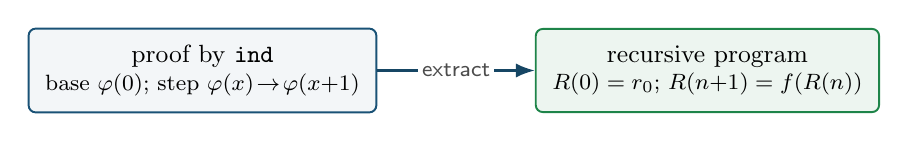
\begin{tikzpicture}[node distance=20mm]
  \node[box,align=center](p){proof by \code{ind}\\[-1pt]\footnotesize base $\varphi(0)$; step $\varphi(x)\!\to\!\varphi(x{+}1)$};
  \node[boxg,align=center,right=of p](r){recursive program\\[-1pt]\footnotesize $R(0)=r_0$; $R(n{+}1)=f(R(n))$};
  \draw[flow](p)--node[elabel]{$\extract$}(r);
\end{tikzpicture}
\caption{Extraction turns the base and step of an induction into the base and
step of a recursion. The stronger induction of Goodstein (below) turns, by the
same move, into a stronger recursion.}
\label{fig:indrec}
\end{figure}

\subsection*{New capability: a structured witness (Towers of Hanoi)}

The Towers of Hanoi puzzle asks for a sequence of moves transferring $n$ disks
between pegs. The fragment proves such a sequence always exists --- and, in the
same breath, that it has exactly $2^n-1$ moves. What is new is the \emph{shape}
of the witness. In Act~II the witness was a bare number, $5$. Here the thing
whose existence we prove is a whole \emph{sequence of moves} --- structured
data, encoded as a number but meaning a list. When $\extract$ runs, the
realizer's witness is that move sequence, and it decodes into a readable list
of ``move a disk from this peg to that peg'' instructions --- the classical
optimal solution, produced by the extracted program and checked to be exactly
the moves a human would write. The existential machine of Act~II, unchanged,
now returns structured data. (The proof uses \code{ind} on the disk count, so
it extracts to a recursion; the recursion branches --- two smaller sub-towers
joined by one move --- which is why the count comes out $2^n-1$.)

Every recursion in this act halts for the same underlying reason, and it is
worth naming that reason once, here, where it is easiest to see. The disk count
is a \emph{descent certificate}: a quantity that strictly drops at every
recursive call and, being a natural number, cannot drop forever
(Figure~\ref{fig:desc-hanoi}). Each example below carries one; watch what it is.

\begin{figure}[h]
\centering
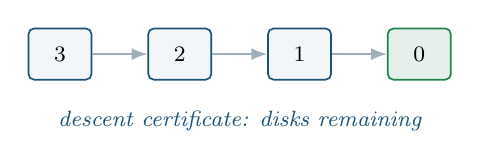
\begin{tikzpicture}[node distance=7mm]
  \node[dbox](a){$3$};
  \node[dbox,right=of a](b){$2$};
  \node[dbox,right=of b](c){$1$};
  \node[dzero,right=of c](d){$0$};
  \foreach \x/\y in {a/b,b/c,c/d} \draw[ladder](\x)--(\y);
  \coordinate (mid) at ($(a)!0.5!(d)$);
  \node[dlab,below=6mm of mid]{descent certificate: disks remaining};
\end{tikzpicture}
\caption{\textbf{Why recursion terminates (Hanoi).} Each recursive call solves a
tower of strictly fewer disks, so the disk count --- the \emph{descent
certificate} --- falls to $0$ and can fall no further. The recursion
\emph{branches} (two sub-towers per disk), but every branch drops the count, so
the whole tree of calls is finite.}
\label{fig:desc-hanoi}
\end{figure}

\subsection*{New capability: a decision procedure (Pascal's triangle, mod $2$)}

Replace every entry of Pascal's triangle by its remainder mod $2$: every number
becomes a $0$ or a $1$. The fragment proves, for each position, that its parity
is $0$ or $1$ --- and, more to the point, \emph{which}. The new capability is
that the extracted program is a \textbf{classifier}. The statement is a
disjunction, ``this entry is $0$, or it is $1$,'' so (Table~\ref{tab:realizers})
its realizer carries a tag naming the answer. Run $\extract$ and that tag
becomes a runnable function from a position to its parity --- a decision
procedure, produced not by us writing one but by extracting it from a proof
that merely said ``the answer is one or the other.'' Tabulate that classifier's
outputs --- a mark for $1$, a blank for $0$, row by row --- and the picture that
appears is the Sierpi\'nski triangle (Figure~\ref{fig:sierpinski}). There is no
gap between the picture and the theorem: every cell of the drawing is one
instance of the proved disjunction, its value filled in by the extracted
realizer's own tag.

\begin{figure}[h]
\centering
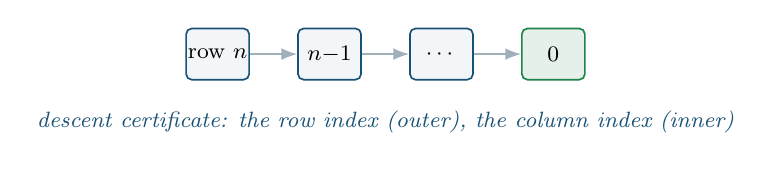
\begin{tikzpicture}[node distance=6mm]
  \node[dbox](a){row $n$};
  \node[dbox,right=of a](b){$n{-}1$};
  \node[dbox,right=of b](c){$\cdots$};
  \node[dzero,right=of c](d){$0$};
  \foreach \x/\y in {a/b,b/c,c/d} \draw[ladder](\x)--(\y);
  \coordinate (mid) at ($(a)!0.5!(d)$);
  \node[dlab,below=6mm of mid]{descent certificate: the row index (outer), the column index (inner)};
\end{tikzpicture}
\caption{\textbf{Why recursion terminates (Pascal).} The proof is a
\emph{nested} induction: the outer recursion descends the row index, and within
each row an inner recursion descends the column index. Two descent
certificates, both ordinary natural numbers, one inside the other.}
\label{fig:desc-pascal}
\end{figure}

\begin{figure}[h]
\centering
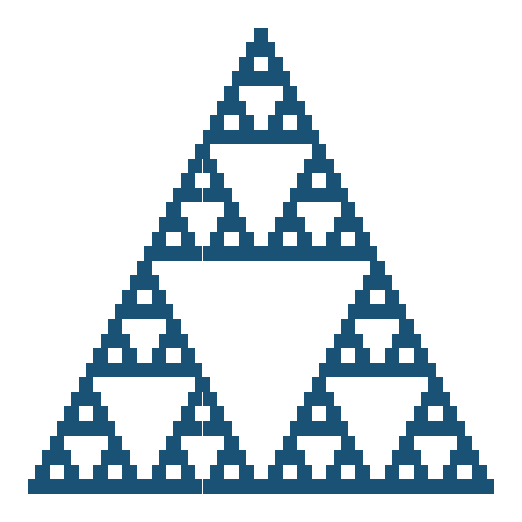
\begin{tikzpicture}
% Pascal's triangle mod 2, rows 0-31, computed by the recurrence
% pas(n,k)=pas(n-1,k-1) XOR pas(n-1,k) and cross-checked against C(n,k) mod 2.
% 243 filled cells (= 3^5). Regenerate with scratchpad/sierp.py.
% 243 filled cells, 32 rows, cell 0.185cm
\fill[accent](0.000,0.000) rectangle ++(0.185,0.185);
\fill[accent](-0.092,-0.185) rectangle ++(0.185,0.185);
\fill[accent](0.092,-0.185) rectangle ++(0.185,0.185);
\fill[accent](-0.185,-0.370) rectangle ++(0.185,0.185);
\fill[accent](0.185,-0.370) rectangle ++(0.185,0.185);
\fill[accent](-0.277,-0.555) rectangle ++(0.185,0.185);
\fill[accent](-0.092,-0.555) rectangle ++(0.185,0.185);
\fill[accent](0.092,-0.555) rectangle ++(0.185,0.185);
\fill[accent](0.277,-0.555) rectangle ++(0.185,0.185);
\fill[accent](-0.370,-0.740) rectangle ++(0.185,0.185);
\fill[accent](0.370,-0.740) rectangle ++(0.185,0.185);
\fill[accent](-0.463,-0.925) rectangle ++(0.185,0.185);
\fill[accent](-0.277,-0.925) rectangle ++(0.185,0.185);
\fill[accent](0.277,-0.925) rectangle ++(0.185,0.185);
\fill[accent](0.463,-0.925) rectangle ++(0.185,0.185);
\fill[accent](-0.555,-1.110) rectangle ++(0.185,0.185);
\fill[accent](-0.185,-1.110) rectangle ++(0.185,0.185);
\fill[accent](0.185,-1.110) rectangle ++(0.185,0.185);
\fill[accent](0.555,-1.110) rectangle ++(0.185,0.185);
\fill[accent](-0.647,-1.295) rectangle ++(0.185,0.185);
\fill[accent](-0.463,-1.295) rectangle ++(0.185,0.185);
\fill[accent](-0.277,-1.295) rectangle ++(0.185,0.185);
\fill[accent](-0.092,-1.295) rectangle ++(0.185,0.185);
\fill[accent](0.092,-1.295) rectangle ++(0.185,0.185);
\fill[accent](0.277,-1.295) rectangle ++(0.185,0.185);
\fill[accent](0.463,-1.295) rectangle ++(0.185,0.185);
\fill[accent](0.647,-1.295) rectangle ++(0.185,0.185);
\fill[accent](-0.740,-1.480) rectangle ++(0.185,0.185);
\fill[accent](0.740,-1.480) rectangle ++(0.185,0.185);
\fill[accent](-0.833,-1.665) rectangle ++(0.185,0.185);
\fill[accent](-0.647,-1.665) rectangle ++(0.185,0.185);
\fill[accent](0.647,-1.665) rectangle ++(0.185,0.185);
\fill[accent](0.833,-1.665) rectangle ++(0.185,0.185);
\fill[accent](-0.925,-1.850) rectangle ++(0.185,0.185);
\fill[accent](-0.555,-1.850) rectangle ++(0.185,0.185);
\fill[accent](0.555,-1.850) rectangle ++(0.185,0.185);
\fill[accent](0.925,-1.850) rectangle ++(0.185,0.185);
\fill[accent](-1.018,-2.035) rectangle ++(0.185,0.185);
\fill[accent](-0.833,-2.035) rectangle ++(0.185,0.185);
\fill[accent](-0.647,-2.035) rectangle ++(0.185,0.185);
\fill[accent](-0.463,-2.035) rectangle ++(0.185,0.185);
\fill[accent](0.463,-2.035) rectangle ++(0.185,0.185);
\fill[accent](0.647,-2.035) rectangle ++(0.185,0.185);
\fill[accent](0.833,-2.035) rectangle ++(0.185,0.185);
\fill[accent](1.018,-2.035) rectangle ++(0.185,0.185);
\fill[accent](-1.110,-2.220) rectangle ++(0.185,0.185);
\fill[accent](-0.370,-2.220) rectangle ++(0.185,0.185);
\fill[accent](0.370,-2.220) rectangle ++(0.185,0.185);
\fill[accent](1.110,-2.220) rectangle ++(0.185,0.185);
\fill[accent](-1.202,-2.405) rectangle ++(0.185,0.185);
\fill[accent](-1.018,-2.405) rectangle ++(0.185,0.185);
\fill[accent](-0.463,-2.405) rectangle ++(0.185,0.185);
\fill[accent](-0.277,-2.405) rectangle ++(0.185,0.185);
\fill[accent](0.277,-2.405) rectangle ++(0.185,0.185);
\fill[accent](0.463,-2.405) rectangle ++(0.185,0.185);
\fill[accent](1.018,-2.405) rectangle ++(0.185,0.185);
\fill[accent](1.202,-2.405) rectangle ++(0.185,0.185);
\fill[accent](-1.295,-2.590) rectangle ++(0.185,0.185);
\fill[accent](-0.925,-2.590) rectangle ++(0.185,0.185);
\fill[accent](-0.555,-2.590) rectangle ++(0.185,0.185);
\fill[accent](-0.185,-2.590) rectangle ++(0.185,0.185);
\fill[accent](0.185,-2.590) rectangle ++(0.185,0.185);
\fill[accent](0.555,-2.590) rectangle ++(0.185,0.185);
\fill[accent](0.925,-2.590) rectangle ++(0.185,0.185);
\fill[accent](1.295,-2.590) rectangle ++(0.185,0.185);
\fill[accent](-1.387,-2.775) rectangle ++(0.185,0.185);
\fill[accent](-1.202,-2.775) rectangle ++(0.185,0.185);
\fill[accent](-1.018,-2.775) rectangle ++(0.185,0.185);
\fill[accent](-0.833,-2.775) rectangle ++(0.185,0.185);
\fill[accent](-0.647,-2.775) rectangle ++(0.185,0.185);
\fill[accent](-0.463,-2.775) rectangle ++(0.185,0.185);
\fill[accent](-0.277,-2.775) rectangle ++(0.185,0.185);
\fill[accent](-0.092,-2.775) rectangle ++(0.185,0.185);
\fill[accent](0.092,-2.775) rectangle ++(0.185,0.185);
\fill[accent](0.277,-2.775) rectangle ++(0.185,0.185);
\fill[accent](0.463,-2.775) rectangle ++(0.185,0.185);
\fill[accent](0.647,-2.775) rectangle ++(0.185,0.185);
\fill[accent](0.833,-2.775) rectangle ++(0.185,0.185);
\fill[accent](1.018,-2.775) rectangle ++(0.185,0.185);
\fill[accent](1.202,-2.775) rectangle ++(0.185,0.185);
\fill[accent](1.387,-2.775) rectangle ++(0.185,0.185);
\fill[accent](-1.480,-2.960) rectangle ++(0.185,0.185);
\fill[accent](1.480,-2.960) rectangle ++(0.185,0.185);
\fill[accent](-1.573,-3.145) rectangle ++(0.185,0.185);
\fill[accent](-1.387,-3.145) rectangle ++(0.185,0.185);
\fill[accent](1.387,-3.145) rectangle ++(0.185,0.185);
\fill[accent](1.573,-3.145) rectangle ++(0.185,0.185);
\fill[accent](-1.665,-3.330) rectangle ++(0.185,0.185);
\fill[accent](-1.295,-3.330) rectangle ++(0.185,0.185);
\fill[accent](1.295,-3.330) rectangle ++(0.185,0.185);
\fill[accent](1.665,-3.330) rectangle ++(0.185,0.185);
\fill[accent](-1.758,-3.515) rectangle ++(0.185,0.185);
\fill[accent](-1.573,-3.515) rectangle ++(0.185,0.185);
\fill[accent](-1.387,-3.515) rectangle ++(0.185,0.185);
\fill[accent](-1.202,-3.515) rectangle ++(0.185,0.185);
\fill[accent](1.202,-3.515) rectangle ++(0.185,0.185);
\fill[accent](1.387,-3.515) rectangle ++(0.185,0.185);
\fill[accent](1.573,-3.515) rectangle ++(0.185,0.185);
\fill[accent](1.758,-3.515) rectangle ++(0.185,0.185);
\fill[accent](-1.850,-3.700) rectangle ++(0.185,0.185);
\fill[accent](-1.110,-3.700) rectangle ++(0.185,0.185);
\fill[accent](1.110,-3.700) rectangle ++(0.185,0.185);
\fill[accent](1.850,-3.700) rectangle ++(0.185,0.185);
\fill[accent](-1.942,-3.885) rectangle ++(0.185,0.185);
\fill[accent](-1.758,-3.885) rectangle ++(0.185,0.185);
\fill[accent](-1.202,-3.885) rectangle ++(0.185,0.185);
\fill[accent](-1.018,-3.885) rectangle ++(0.185,0.185);
\fill[accent](1.018,-3.885) rectangle ++(0.185,0.185);
\fill[accent](1.202,-3.885) rectangle ++(0.185,0.185);
\fill[accent](1.758,-3.885) rectangle ++(0.185,0.185);
\fill[accent](1.942,-3.885) rectangle ++(0.185,0.185);
\fill[accent](-2.035,-4.070) rectangle ++(0.185,0.185);
\fill[accent](-1.665,-4.070) rectangle ++(0.185,0.185);
\fill[accent](-1.295,-4.070) rectangle ++(0.185,0.185);
\fill[accent](-0.925,-4.070) rectangle ++(0.185,0.185);
\fill[accent](0.925,-4.070) rectangle ++(0.185,0.185);
\fill[accent](1.295,-4.070) rectangle ++(0.185,0.185);
\fill[accent](1.665,-4.070) rectangle ++(0.185,0.185);
\fill[accent](2.035,-4.070) rectangle ++(0.185,0.185);
\fill[accent](-2.127,-4.255) rectangle ++(0.185,0.185);
\fill[accent](-1.942,-4.255) rectangle ++(0.185,0.185);
\fill[accent](-1.758,-4.255) rectangle ++(0.185,0.185);
\fill[accent](-1.573,-4.255) rectangle ++(0.185,0.185);
\fill[accent](-1.387,-4.255) rectangle ++(0.185,0.185);
\fill[accent](-1.202,-4.255) rectangle ++(0.185,0.185);
\fill[accent](-1.018,-4.255) rectangle ++(0.185,0.185);
\fill[accent](-0.833,-4.255) rectangle ++(0.185,0.185);
\fill[accent](0.833,-4.255) rectangle ++(0.185,0.185);
\fill[accent](1.018,-4.255) rectangle ++(0.185,0.185);
\fill[accent](1.202,-4.255) rectangle ++(0.185,0.185);
\fill[accent](1.387,-4.255) rectangle ++(0.185,0.185);
\fill[accent](1.573,-4.255) rectangle ++(0.185,0.185);
\fill[accent](1.758,-4.255) rectangle ++(0.185,0.185);
\fill[accent](1.942,-4.255) rectangle ++(0.185,0.185);
\fill[accent](2.127,-4.255) rectangle ++(0.185,0.185);
\fill[accent](-2.220,-4.440) rectangle ++(0.185,0.185);
\fill[accent](-0.740,-4.440) rectangle ++(0.185,0.185);
\fill[accent](0.740,-4.440) rectangle ++(0.185,0.185);
\fill[accent](2.220,-4.440) rectangle ++(0.185,0.185);
\fill[accent](-2.312,-4.625) rectangle ++(0.185,0.185);
\fill[accent](-2.127,-4.625) rectangle ++(0.185,0.185);
\fill[accent](-0.833,-4.625) rectangle ++(0.185,0.185);
\fill[accent](-0.647,-4.625) rectangle ++(0.185,0.185);
\fill[accent](0.647,-4.625) rectangle ++(0.185,0.185);
\fill[accent](0.833,-4.625) rectangle ++(0.185,0.185);
\fill[accent](2.127,-4.625) rectangle ++(0.185,0.185);
\fill[accent](2.312,-4.625) rectangle ++(0.185,0.185);
\fill[accent](-2.405,-4.810) rectangle ++(0.185,0.185);
\fill[accent](-2.035,-4.810) rectangle ++(0.185,0.185);
\fill[accent](-0.925,-4.810) rectangle ++(0.185,0.185);
\fill[accent](-0.555,-4.810) rectangle ++(0.185,0.185);
\fill[accent](0.555,-4.810) rectangle ++(0.185,0.185);
\fill[accent](0.925,-4.810) rectangle ++(0.185,0.185);
\fill[accent](2.035,-4.810) rectangle ++(0.185,0.185);
\fill[accent](2.405,-4.810) rectangle ++(0.185,0.185);
\fill[accent](-2.498,-4.995) rectangle ++(0.185,0.185);
\fill[accent](-2.312,-4.995) rectangle ++(0.185,0.185);
\fill[accent](-2.127,-4.995) rectangle ++(0.185,0.185);
\fill[accent](-1.942,-4.995) rectangle ++(0.185,0.185);
\fill[accent](-1.018,-4.995) rectangle ++(0.185,0.185);
\fill[accent](-0.833,-4.995) rectangle ++(0.185,0.185);
\fill[accent](-0.647,-4.995) rectangle ++(0.185,0.185);
\fill[accent](-0.463,-4.995) rectangle ++(0.185,0.185);
\fill[accent](0.463,-4.995) rectangle ++(0.185,0.185);
\fill[accent](0.647,-4.995) rectangle ++(0.185,0.185);
\fill[accent](0.833,-4.995) rectangle ++(0.185,0.185);
\fill[accent](1.018,-4.995) rectangle ++(0.185,0.185);
\fill[accent](1.942,-4.995) rectangle ++(0.185,0.185);
\fill[accent](2.127,-4.995) rectangle ++(0.185,0.185);
\fill[accent](2.312,-4.995) rectangle ++(0.185,0.185);
\fill[accent](2.498,-4.995) rectangle ++(0.185,0.185);
\fill[accent](-2.590,-5.180) rectangle ++(0.185,0.185);
\fill[accent](-1.850,-5.180) rectangle ++(0.185,0.185);
\fill[accent](-1.110,-5.180) rectangle ++(0.185,0.185);
\fill[accent](-0.370,-5.180) rectangle ++(0.185,0.185);
\fill[accent](0.370,-5.180) rectangle ++(0.185,0.185);
\fill[accent](1.110,-5.180) rectangle ++(0.185,0.185);
\fill[accent](1.850,-5.180) rectangle ++(0.185,0.185);
\fill[accent](2.590,-5.180) rectangle ++(0.185,0.185);
\fill[accent](-2.683,-5.365) rectangle ++(0.185,0.185);
\fill[accent](-2.498,-5.365) rectangle ++(0.185,0.185);
\fill[accent](-1.942,-5.365) rectangle ++(0.185,0.185);
\fill[accent](-1.758,-5.365) rectangle ++(0.185,0.185);
\fill[accent](-1.202,-5.365) rectangle ++(0.185,0.185);
\fill[accent](-1.018,-5.365) rectangle ++(0.185,0.185);
\fill[accent](-0.463,-5.365) rectangle ++(0.185,0.185);
\fill[accent](-0.277,-5.365) rectangle ++(0.185,0.185);
\fill[accent](0.277,-5.365) rectangle ++(0.185,0.185);
\fill[accent](0.463,-5.365) rectangle ++(0.185,0.185);
\fill[accent](1.018,-5.365) rectangle ++(0.185,0.185);
\fill[accent](1.202,-5.365) rectangle ++(0.185,0.185);
\fill[accent](1.758,-5.365) rectangle ++(0.185,0.185);
\fill[accent](1.942,-5.365) rectangle ++(0.185,0.185);
\fill[accent](2.498,-5.365) rectangle ++(0.185,0.185);
\fill[accent](2.683,-5.365) rectangle ++(0.185,0.185);
\fill[accent](-2.775,-5.550) rectangle ++(0.185,0.185);
\fill[accent](-2.405,-5.550) rectangle ++(0.185,0.185);
\fill[accent](-2.035,-5.550) rectangle ++(0.185,0.185);
\fill[accent](-1.665,-5.550) rectangle ++(0.185,0.185);
\fill[accent](-1.295,-5.550) rectangle ++(0.185,0.185);
\fill[accent](-0.925,-5.550) rectangle ++(0.185,0.185);
\fill[accent](-0.555,-5.550) rectangle ++(0.185,0.185);
\fill[accent](-0.185,-5.550) rectangle ++(0.185,0.185);
\fill[accent](0.185,-5.550) rectangle ++(0.185,0.185);
\fill[accent](0.555,-5.550) rectangle ++(0.185,0.185);
\fill[accent](0.925,-5.550) rectangle ++(0.185,0.185);
\fill[accent](1.295,-5.550) rectangle ++(0.185,0.185);
\fill[accent](1.665,-5.550) rectangle ++(0.185,0.185);
\fill[accent](2.035,-5.550) rectangle ++(0.185,0.185);
\fill[accent](2.405,-5.550) rectangle ++(0.185,0.185);
\fill[accent](2.775,-5.550) rectangle ++(0.185,0.185);
\fill[accent](-2.868,-5.735) rectangle ++(0.185,0.185);
\fill[accent](-2.683,-5.735) rectangle ++(0.185,0.185);
\fill[accent](-2.498,-5.735) rectangle ++(0.185,0.185);
\fill[accent](-2.312,-5.735) rectangle ++(0.185,0.185);
\fill[accent](-2.127,-5.735) rectangle ++(0.185,0.185);
\fill[accent](-1.942,-5.735) rectangle ++(0.185,0.185);
\fill[accent](-1.758,-5.735) rectangle ++(0.185,0.185);
\fill[accent](-1.573,-5.735) rectangle ++(0.185,0.185);
\fill[accent](-1.387,-5.735) rectangle ++(0.185,0.185);
\fill[accent](-1.202,-5.735) rectangle ++(0.185,0.185);
\fill[accent](-1.018,-5.735) rectangle ++(0.185,0.185);
\fill[accent](-0.833,-5.735) rectangle ++(0.185,0.185);
\fill[accent](-0.647,-5.735) rectangle ++(0.185,0.185);
\fill[accent](-0.463,-5.735) rectangle ++(0.185,0.185);
\fill[accent](-0.277,-5.735) rectangle ++(0.185,0.185);
\fill[accent](-0.092,-5.735) rectangle ++(0.185,0.185);
\fill[accent](0.092,-5.735) rectangle ++(0.185,0.185);
\fill[accent](0.277,-5.735) rectangle ++(0.185,0.185);
\fill[accent](0.463,-5.735) rectangle ++(0.185,0.185);
\fill[accent](0.647,-5.735) rectangle ++(0.185,0.185);
\fill[accent](0.833,-5.735) rectangle ++(0.185,0.185);
\fill[accent](1.018,-5.735) rectangle ++(0.185,0.185);
\fill[accent](1.202,-5.735) rectangle ++(0.185,0.185);
\fill[accent](1.387,-5.735) rectangle ++(0.185,0.185);
\fill[accent](1.573,-5.735) rectangle ++(0.185,0.185);
\fill[accent](1.758,-5.735) rectangle ++(0.185,0.185);
\fill[accent](1.942,-5.735) rectangle ++(0.185,0.185);
\fill[accent](2.127,-5.735) rectangle ++(0.185,0.185);
\fill[accent](2.312,-5.735) rectangle ++(0.185,0.185);
\fill[accent](2.498,-5.735) rectangle ++(0.185,0.185);
\fill[accent](2.683,-5.735) rectangle ++(0.185,0.185);
\fill[accent](2.868,-5.735) rectangle ++(0.185,0.185);

\end{tikzpicture}
\caption{The extracted classifier's own output, rows $0$--$31$: a filled cell
where the decided parity is $1$, blank where it is $0$. The Sierpi\'nski
triangle here is not a picture drawn to resemble the theorem --- it \emph{is}
the theorem, one cell per proved instance of ``this entry is $0$ or $1$,'' each
cell's value read off the extracted realizer's tag. Generated from the parity
recurrence $\mathrm{pas}(n,k)=\mathrm{pas}(n{-}1,k{-}1)\oplus\mathrm{pas}(n{-}1,k)$
and cross-checked against $\binom{n}{k}\bmod 2$; the $243=3^5$ filled cells over
$32$ rows are exactly the count the closed form predicts.}
\label{fig:sierpinski}
\end{figure}

\subsection*{New capability: a strengthened induction hypothesis (Fibonacci)}

The Fibonacci numbers $0,1,1,2,3,5,8,\dots$ are each the sum of the previous
two. Suppose we want to prove, in a form from which we can extract a program,
that $\fib$ is total. Try it by ordinary induction and you hit a wall worth
feeling: induction hands you the statement \emph{at $n$}, but computing
$\fib(n+2)$ needs \emph{two} earlier values, $\fib(n+1)$ and $\fib(n)$, and the
hypothesis at $n$ alone does not give both. The new capability is the standard
cure. Instead of proving ``$\fib(n)$ exists,'' prove the stronger pair
statement: the \emph{pair} $\bigl(\fib(n),\fib(n+1)\bigr)$ exists. Now the
hypothesis hands you both consecutive values, and the step is a single shift,
\[
  \bigl(\fib(n),\ \fib(n+1)\bigr)\ \longmapsto\
  \bigl(\fib(n+1),\ \fib(n)+\fib(n+1)\bigr).
\]
A stronger hypothesis is a stronger thing to be handed at the step, so the
induction goes through. Extract that proof and --- exactly as
Figure~\ref{fig:indrec} predicts --- you get the fast two-variable iterative
Fibonacci every programmer knows: carry a pair, shift it $n$ times, read off a
component. The proof's strengthened hypothesis \emph{is} the program's pair of
accumulator variables; you can watch the extracted pair advance through
$(0,1),(1,1),(1,2),(2,3)$ --- the loop's running state, read out of a proof
that never mentions a loop.

\begin{figure}[h]
\centering
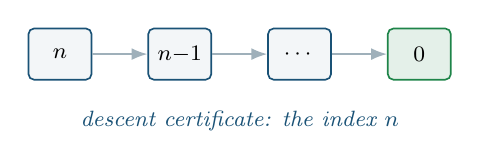
\begin{tikzpicture}[node distance=7mm]
  \node[dbox](a){$n$};
  \node[dbox,right=of a](b){$n{-}1$};
  \node[dbox,right=of b](c){$\cdots$};
  \node[dzero,right=of c](d){$0$};
  \foreach \x/\y in {a/b,b/c,c/d} \draw[ladder](\x)--(\y);
  \coordinate (mid) at ($(a)!0.5!(d)$);
  \node[dlab,below=6mm of mid]{descent certificate: the index $n$};
\end{tikzpicture}
\caption{\textbf{Why recursion terminates (Fibonacci).} Strengthening the
hypothesis to a pair changed what is \emph{carried} at each step --- the two
accumulators --- not what makes the recursion stop. The descent certificate is
still the plain index $n$, counting down to $0$.}
\label{fig:desc-fib}
\end{figure}

\subsection*{New capability: taming variable capture (Euclid's gcd)}

The fragment proves that any two numbers have a greatest common divisor --- and
the extracted witness \emph{is} the gcd, computed by subtractive Euclid
(repeatedly replace the larger number by the difference), with no gcd operation
built into the fragment. Two supporting economies make this possible. First,
the fragment never added an ``order'' operation: $s<t$ is simply $\exists d.\
(s+1)+d=t$ --- order is an existential over addition, not a primitive. Second,
it never added ``strong induction'' (where the step may use \emph{all} smaller
cases); that is \emph{derived} from ordinary \code{ind}.

But the new capability the gcd proof forces is neither of these --- it is a
problem about \emph{substitution}. When you instantiate an induction hypothesis
or a ``for all,'' you substitute a term for a bound variable; if that term
mentions a variable that is \emph{also} bound in the formula, the substitution
silently confuses two different variables sharing a name --- the notorious
\emph{variable capture}. The fragment's substitution is deliberately
simple-minded: rather than quietly renaming to avoid capture, it \emph{forbids}
the capturing substitution outright, so the proof author must route around it.
Euclid's recursion is the first place two capture problems bite at once, and the
first to use the fragment's two general-purpose dodges \emph{together}: give the
offending term a fresh name with an extra ``for all'' and instantiate at the
harmless name; and, when a recursion permutes its arguments, rename those
variables to fresh ones first. Neither changes what is proved or what the
program computes; both merely coax a naive substitution system into accepting a
substitution that is morally fine. Out the far end comes a certified
greatest-common-divisor calculator --- which, pleasingly, needs no special case
for zero: the specification is met by $\gcd(0,0)=0$, since everything divides
$0$.

\begin{figure}[h]
\centering
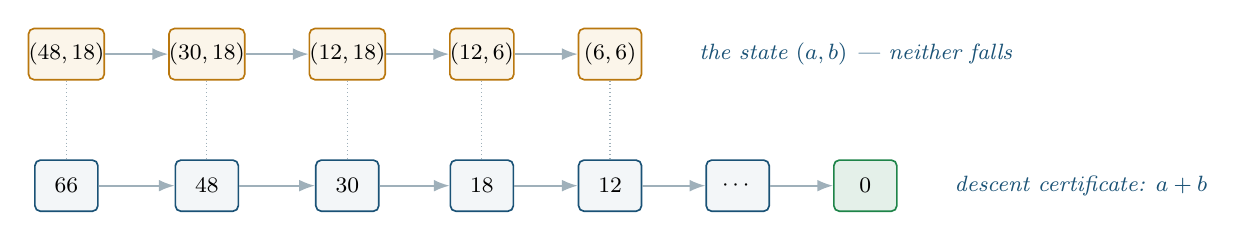
\begin{tikzpicture}[node distance=5.5mm and 8mm]
  \node[dup](p0){$(48,18)$};
  \node[dup,right=of p0](p1){$(30,18)$};
  \node[dup,right=of p1](p2){$(12,18)$};
  \node[dup,right=of p2](p3){$(12,6)$};
  \node[dup,right=of p3](p4){$(6,6)$};
  \foreach \x/\y in {p0/p1,p1/p2,p2/p3,p3/p4} \draw[ladder](\x)--(\y);
  \node[dbox,below=10mm of p0](s0){$66$};
  \node[dbox,below=10mm of p1](s1){$48$};
  \node[dbox,below=10mm of p2](s2){$30$};
  \node[dbox,below=10mm of p3](s3){$18$};
  \node[dbox,below=10mm of p4](s4){$12$};
  \node[dbox,right=of s4](s5){$\cdots$};
  \node[dzero,right=of s5](s6){$0$};
  \foreach \x/\y in {s0/s1,s1/s2,s2/s3,s3/s4,s4/s5,s5/s6} \draw[ladder](\x)--(\y);
  \foreach \p in {p0,p1,p2,p3,p4} \draw[densely dotted,draw=rulec](\p)--(\p|-s0.north);
  \node[dlab,right=6mm of p4]{the state $(a,b)$ --- neither falls};
  \node[dlab,right=6mm of s6]{descent certificate: $a+b$};
\end{tikzpicture}
\caption{\textbf{Why recursion terminates (Euclid).} Subtractive Euclid replaces
the larger number by the difference. Neither coordinate of the pair (amber)
falls at every step --- but their \emph{sum} (below) does, strictly, until it
reaches $0$. The descent certificate here is not one of the arguments; it is the
derived quantity $a+b$, which is exactly why the proof runs a course-of-values
(``strong'') induction \emph{on the sum} rather than on either number.}
\label{fig:desc-euclid}
\end{figure}

\subsection*{New capability: more general than the classical statement (Sperner, 1D)}

Colour the points $0,1,\dots,n$ along a line, each some natural-number colour,
with the two ends coloured differently. Then somewhere two \emph{adjacent}
points must differ --- you cannot get from one end-colour to the other without a
change. This is the one-dimensional Sperner lemma~\citep{sperner1928}, the
discrete ancestor of the intermediate value theorem. The fragment proves it by ordinary induction,
scanning the line and carrying ``either we are still at the start colour, or we
have already found a crossing''; the extracted program is a left-to-right search
returning the \emph{first} crossing. But the new thing is not the extraction ---
it is the theorem. The classical statement is usually given for \emph{two}
colours; the fragment's proof never uses that restriction. It works for
\emph{arbitrary} natural-number colourings, so the extracted search is more
general than the classical picture. The proof turned out to prove \emph{more}
than the theorem it was written for.

\begin{figure}[h]
\centering
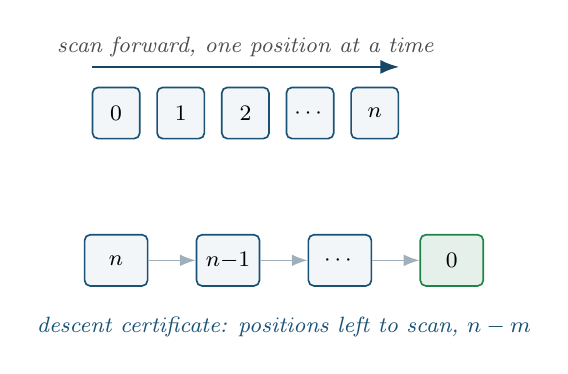
\begin{tikzpicture}[node distance=6mm]
  \node[dbox,minimum width=6mm](c0){$0$};
  \node[dbox,minimum width=6mm,right=2mm of c0](c1){$1$};
  \node[dbox,minimum width=6mm,right=2mm of c1](c2){$2$};
  \node[dbox,minimum width=6mm,right=2mm of c2](c3){$\cdots$};
  \node[dbox,minimum width=6mm,right=2mm of c3](c4){$n$};
  \draw[flow] ([yshift=2.5mm]c0.north west) -- ([yshift=2.5mm]c4.north east)
     node[midway,above,font=\footnotesize\itshape,text=black!70]{scan forward, one position at a time};
  \node[dbox,below=12mm of c0](r0){$n$};
  \node[dbox,right=of r0](r1){$n{-}1$};
  \node[dbox,right=of r1](r2){$\cdots$};
  \node[dzero,right=of r2](r3){$0$};
  \foreach \x/\y in {r0/r1,r1/r2,r2/r3} \draw[ladder](\x)--(\y);
  \coordinate (mid) at ($(r0)!0.5!(r3)$);
  \node[dlab,below=6mm of mid]{descent certificate: positions left to scan, $n-m$};
\end{tikzpicture}
\caption{\textbf{Why recursion terminates (Sperner).} The extracted program is a
\emph{forward linear scan}: it walks the points $0,1,\dots,n$ left to right,
stopping at the first colour change. The descent certificate is the number of
unscanned positions, $n-m$, dropping by exactly one per step --- a straight walk
to the end, not an interval halved by bisection.}
\label{fig:desc-sperner}
\end{figure}

\subsection*{New capability: recursion along the ordinals (Goodstein)}

Now Goodstein itself, the general theorem behind Act~II's single hand-worked
case. Act~II proved $\exists s.\ \good(3,s)=0$ with the witness supplied by us
as $5$. Goodstein's \emph{theorem} is the universal version,
\[
  \forall m.\ \exists s.\ \good(m,s)=0,
\]
and we want from it the same thing Act~II gave, but uniform in $m$: a program
that, given $m$, returns the stopping step. The proof cannot know $m$'s answer
in advance, so the witness must be \emph{produced} by the proof.

Every example so far has handed us a descent certificate that was an ordinary
natural number --- a disk count, a row index, a plain index, a sum, a count of
positions left to scan. \textbf{Goodstein is where that stops being enough.}
This is the same fact as Act~I's promissory note --- that ordinary induction is
not enough --- now come due: induct on $m$, or $s$, or the value $\good(m,s)$,
and you fail, because the value goes \emph{up} at almost every step, so no
natural-number quantity decreases as the sequence runs. The descent certificate
Goodstein needs is not a natural number at all --- it is the same idea of
descent, reaching one step past the naturals.
To see why, write a number in hereditary base and watch a step act on it:
\[
  13 \;=\; 2^{2+1} + 2^{2} + 1
  \;\;\xrightarrow{\ 2\,\rightsquigarrow\,3\ }\;\;
  3^{3+1} + 3^{3} + 1 \;=\; 109
  \;\;\xrightarrow{\ -1\ }\;\; 108.
\]
Replacing every base $2$ by a $3$ --- \emph{including the ones inside the
exponents} --- inflates $13$ to $108$ in a single step. Yet if you read that
same expression not as a number but as an \emph{ordinal} --- interpret each
base as $\omega$, the first infinity --- the base change does nothing (every
base is already $\omega$), while the ``$-1$'' strictly \emph{lowers} it. Every
Goodstein step, however it inflates the natural-number value, strictly descends
an ordinal below $\epsz$ (epsilon-nought); and the ordinals are
\emph{well-ordered} --- no infinite descending chains
(Figure~\ref{fig:ordinals}) --- so the sequence cannot descend forever and must
reach $0$.
\[
  0 < 1 < 2 < \cdots < \omega < \omega+1 < \cdots < \omega^2 < \cdots
    < \omega^\omega < \cdots < \epsz .
\]
This is the extra strength Act~I warned of: \textbf{transfinite induction up to
$\epsz$}, the single rule in the fragment's whole repertoire that is not a
consequence of ordinary logic and ordinary induction --- it is exactly the
principle Gentzen showed lies beyond ordinary arithmetic~\citep{gentzen1943},
here realized as recursion along a primitive-recursive ordering in the manner
of Tait~\citep{tait1965}. To make it mechanical the
fragment builds the $\epsz$ ordinals \emph{as ordinary numbers} under a
hand-crafted encoding, defines the ``smaller ordinal'' relation on those codes,
and proves --- by elementary means, no infinite reasoning --- that it admits no
infinite descending chain. (Why the encoding was built by hand rather than
borrowed is an Act~VI discovery.)

\begin{figure}[h]
\centering
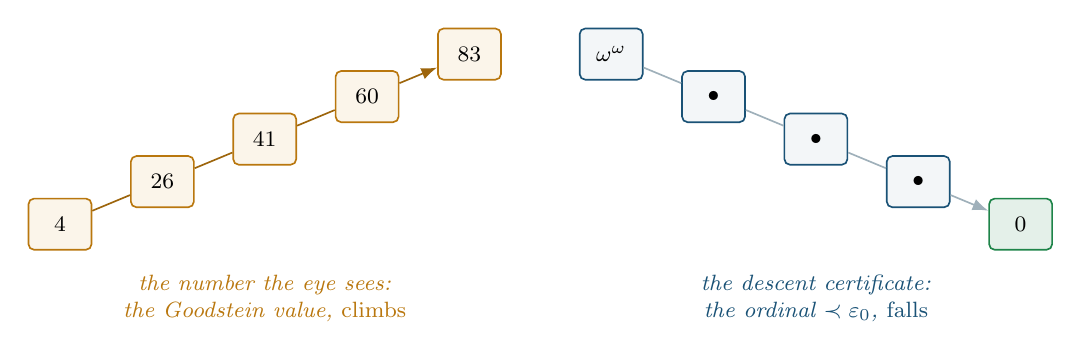
\begin{tikzpicture}[x=13mm,y=9mm,every node/.style={font=\footnotesize}]
  % ---- left: the Goodstein value climbs ----
  \node[dup] (v0) at (0,0)  {$4$};
  \node[dup] (v1) at (1,0.6){$26$};
  \node[dup] (v2) at (2,1.2){$41$};
  \node[dup] (v3) at (3,1.8){$60$};
  \node[dup] (v4) at (4,2.4){$83$};
  \draw[ladder,draw=amber!85!black] (v0)--(v1)--(v2)--(v3)--(v4);
  \node[dlab,text=amber,align=center] at (2,-1.05)
    {the number the eye sees:\\ the Goodstein value, \emph{climbs}};
  % ---- right: the ordinal descends ----
  \begin{scope}[xshift=70mm]
  \node[dbox]  (o0) at (0,2.4){$\omega^{\omega}$};
  \node[dbox]  (o1) at (1,1.8){$\bullet$};
  \node[dbox]  (o2) at (2,1.2){$\bullet$};
  \node[dbox]  (o3) at (3,0.6){$\bullet$};
  \node[dzero] (o4) at (4,0)  {$0$};
  \draw[ladder] (o0)--(o1)--(o2)--(o3)--(o4);
  \node[dlab,align=center] at (2,-1.05)
    {the descent certificate:\\ the ordinal $\prec\epsz$, \emph{falls}};
  \end{scope}
\end{tikzpicture}
\caption{\textbf{Why recursion terminates (Goodstein) --- the signature
contrast.} Starting from $m=4$, the Goodstein value climbs (left; the real
values $4,26,41,60,83,\dots$) while the ordinal assigned to each state (right)
strictly \emph{descends} through the well-order below $\epsz$, from
$\omega^{\omega}$ toward $0$. The intermediate ordinals (shown $\bullet$) are
intricate, but every one lies strictly below the last, and a descending chain of
ordinals cannot run forever. The proof follows the falling certificate on the
right, never the climbing number on the left --- which is why a sequence that
grows can still be proved to stop.}
\label{fig:ordinals}
\end{figure}

Now the two acts line up. In Act~II, $\extract$ turned an existential proof into
a witness by reading a number the proof supplied. Here it turns Goodstein's
proof into a witness by \emph{recursion along the ordinals}: the
transfinite-induction rule extracts to a program that descends the ordinal of
each state until it reaches the bottom, and the number of descents is the
stopping step. Where \code{ind} extracted to ``iterate a step $k$ times''
(Figure~\ref{fig:indrec}), the transfinite rule extracts to ``recur along the
ordinal ordering'' --- a stronger recursion for a stronger induction. Same
machine, one gear higher:
\[
  \forall m.\ \exists s.\ \good(m,s)=0
  \qquad\xrightarrow{\ \extract\ }\qquad
  m \longmapsto s .
\]
One theorem; one extracted program. And it runs (Table~\ref{tab:stop}). The row
for $m=4$ is where Act~I's ``numbers explode'' stops being an assertion: the
program declines to finish because the terminating sequence really is that
long.

\begin{table}[h]
\centering
\renewcommand{\arraystretch}{1.25}
\begin{tabular}{@{}l cccc c c@{}}
\toprule
start $m$          & $0$ & $1$ & $2$ & $3$ & $\cdots$ & $4$ \\
\midrule
stopping step $s$  & $0$ & $1$ & $3$ & $5$ & $\cdots$ & (not attempted) \\
\bottomrule
\end{tabular}
\caption{The extracted stopping-step program $m\mapsto s$. It returns $0$ and
$1$ directly when run; soundness certifies $3$ and $5$ for $m=2,3$ (the
sequences $2,2,1,0$ and $3,3,3,2,1,0$) even where running the program that far
is slow; $m=4$ is not attempted --- its sequence begins $4,26,41,60,\dots$ and
its stopping step is astronomically large.}
\label{tab:stop}
\end{table}

\subsubsection*{An aside: the same function, computed two ways}

That stopping-time function $m\mapsto s$ can be written as a program in two very
different ways, and the difference is exactly the subject of this whole tour. The
obvious way is a \emph{search}: run the sequence, test for zero, return the first
step that hits it --- a \code{while} loop, the classical minimization operator.
It is easy to write and, for small $m$, easy to run. But look at where its
termination lives: the loop halts \emph{if and only if} the sequence really does
reach $0$ --- which is Goodstein's theorem. Nothing inside the loop guarantees
it. The other way is the \emph{extracted} program of Figure~\ref{fig:search}: the
recursion along the descending ordinals we have just described, which halts
\emph{by construction}, because a chain of ordinals below $\epsz$ cannot descend
forever --- no matter how large the natural-number values swell in between.

\begin{figure}[h]
\centering
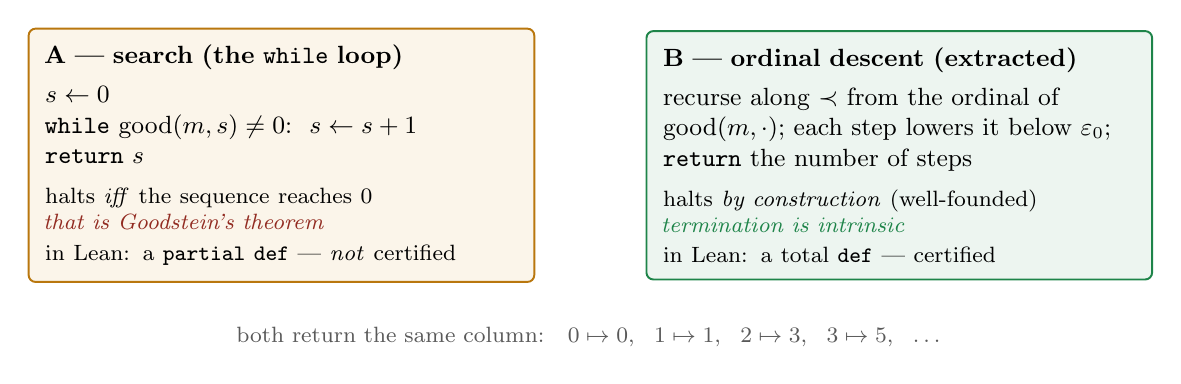
\begin{tikzpicture}[node distance=8mm]
  \node[boxa,text width=60mm,align=left](S){%
    \textbf{A --- search (the \code{while} loop)}\\[3pt]
    $s \gets 0$\\
    \code{while}\ $\good(m,s)\neq 0$:\ \ $s \gets s+1$\\
    \code{return}\ $s$\\[5pt]
    \footnotesize halts \emph{iff} the sequence reaches $0$\\
    \footnotesize {\itshape\color{bad} that is Goodstein's theorem}\\
    \footnotesize in Lean: a \code{partial def} --- \emph{not} certified};
  \node[boxg,text width=60mm,align=left,right=14mm of S](D){%
    \textbf{B --- ordinal descent (extracted)}\\[3pt]
    recurse along $\prec$ from the ordinal of\\
    $\good(m,\cdot)$; each step lowers it below $\epsz$;\\
    \code{return}\ the number of steps\\[5pt]
    \footnotesize halts \emph{by construction} (well-founded)\\
    \footnotesize {\itshape\color{good} termination is intrinsic}\\
    \footnotesize in Lean: a total \code{def} --- certified};
  \node[figcap,align=center] at ($(S.south)!0.5!(D.south) - (0,7mm)$)
    {both return the same column:\ \ \ $0\mapsto 0,\ \ 1\mapsto 1,\ \ 2\mapsto 3,\ \ 3\mapsto 5,\ \ \dots$};
\end{tikzpicture}
\caption{One function, two programs. Both compute the Goodstein stopping time and
agree wherever they run, but their termination guarantees sit in opposite places.
Program A is a search whose halting \emph{is} the theorem: written directly in
Lean it must be marked \code{partial}, the kernel's way of saying ``not certified
to terminate.'' Program B, extracted from the proof, is a total \code{def} whose
halting is carried by the well-founded ordinal descent. The gap is one keyword.}
\label{fig:search}
\end{figure}

The dependency is not merely narrated --- it can be made a proof. Lean's
constructive minimization operator (\code{Nat.find}) turns the search into a
\emph{total} function, but only when handed a proof that a zero exists; and the
one such proof available is the extracted theorem itself.

\begin{keystmt}
The search becomes certified-total exactly by \emph{consuming Goodstein's
theorem} as its termination argument. ``Halts iff the theorem holds'' stops
being a remark and becomes the type of the program.
\end{keystmt}

\noindent
One caveat keeps the picture honest: the certificate buys \emph{termination}, not
\emph{speed}. The certified search still evaluates by running the sequence, so at
$m=4$ it is as unreachable as before --- Program B's guarantee is that it
\emph{will} finish, not that it finishes soon.

\subsection*{New capability: a fragment theorem versus a metatheorem (the Hydra)}

The last and hardest example marks a boundary --- the place where what the
fragment can \emph{prove} and what it can even \emph{state} come apart.

The Hydra is a many-headed tree; Hercules chops a head and it regrows, often
growing \emph{more} heads than it lost. The Kirby--Paris
theorem~\citep{kirbyparis1982} says Hercules wins anyway: every battle
terminates. The reason is Goodstein's in disguise ---
each chop, though it grows the tree, strictly lowers an ordinal below $\epsz$
assigned to it. The fragment can prove termination for \emph{one fixed, encoded
battle}: fix a starting Hydra and a fixed way of playing, code it all as
numbers, and prove $\forall h.\ \exists t.\ \hydra(h,t)=0$ --- the exact shape of
Goodstein's theorem, proved the exact same way, extracting to a battle-length
program. Business as usual --- including the reason it terminates
(Figure~\ref{fig:hydra-desc}).

\begin{figure}[h]
\centering
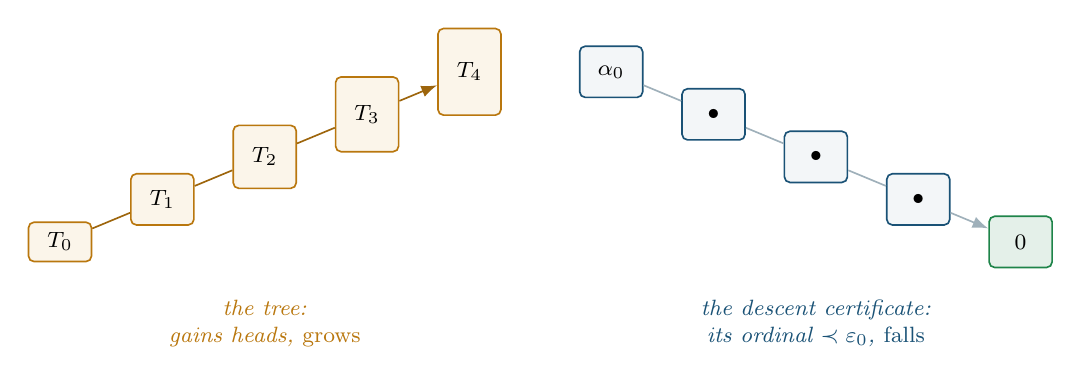
\begin{tikzpicture}[x=13mm,y=9mm,every node/.style={font=\footnotesize}]
  \node[dup,minimum height=5mm]   (t0) at (0,0)  {$T_0$};
  \node[dup,minimum height=6.5mm] (t1) at (1,0.6){$T_1$};
  \node[dup,minimum height=8mm]   (t2) at (2,1.2){$T_2$};
  \node[dup,minimum height=9.5mm] (t3) at (3,1.8){$T_3$};
  \node[dup,minimum height=11mm]  (t4) at (4,2.4){$T_4$};
  \draw[ladder,draw=amber!85!black] (t0)--(t1)--(t2)--(t3)--(t4);
  \node[dlab,text=amber,align=center] at (2,-1.15)
    {the tree:\\ gains heads, \emph{grows}};
  \begin{scope}[xshift=70mm]
  \node[dbox]  (a0) at (0,2.4){$\alpha_0$};
  \node[dbox]  (a1) at (1,1.8){$\bullet$};
  \node[dbox]  (a2) at (2,1.2){$\bullet$};
  \node[dbox]  (a3) at (3,0.6){$\bullet$};
  \node[dzero] (a4) at (4,0)  {$0$};
  \draw[ladder] (a0)--(a1)--(a2)--(a3)--(a4);
  \node[dlab,align=center] at (2,-1.15)
    {the descent certificate:\\ its ordinal $\prec\epsz$, \emph{falls}};
  \end{scope}
\end{tikzpicture}
\caption{\textbf{Why recursion terminates (the Hydra) --- the same signature.}
Each chop regrows the Hydra, usually with \emph{more} heads than before, so the
tree size climbs (left, successive states $T_0,T_1,\dots$). Yet the ordinal
$\alpha_i\prec\epsz$ assigned to each tree strictly falls (right), by exactly
Goodstein's mechanism. Termination follows the ordinal, not the head count ---
the identical shape to Figure~\ref{fig:ordinals}, which is why the fragment
proves it the identical way.}
\label{fig:hydra-desc}
\end{figure}

But the \emph{real} Kirby--Paris theorem says Hercules wins \emph{no matter what
strategy} he uses --- and this the fragment cannot even express
(Figure~\ref{fig:hydra}). To say ``for every strategy'' you must quantify over
strategies, and a strategy is a \emph{function} (it looks at the current Hydra
and decides the next chop). The fragment's ``for all'' ranges only over
\emph{numbers}, never functions. The limitation is not that the fragment fails
to \emph{prove} the general theorem; the sentence expressing it is not in the
fragment's language at all. So the general theorem is proved \emph{outside} the
fragment, in the ordinary mathematics of the proof assistant, which quantifies
over functions freely; and the fragment's single battle is checked to be one of
those general plays, a genuine special case. This split --- a \emph{fragment
theorem} for one battle, a \emph{metatheorem} for all strategies --- is forced,
cleanly and provably, by the one fact that the fragment has no function
variables. It is the right place to stop feeding the machine harder proofs.

\begin{figure}[h]
\centering
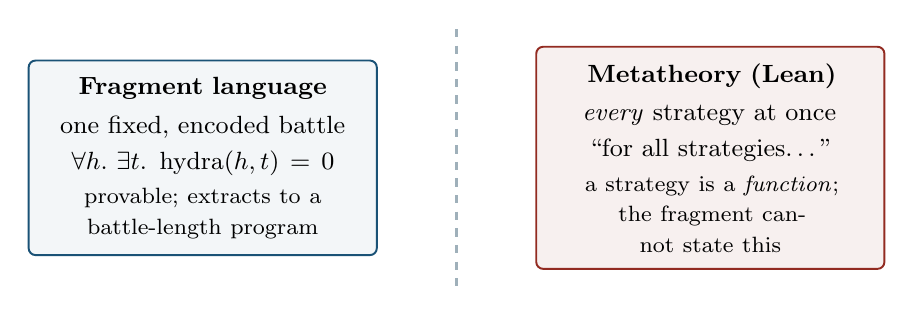
\begin{tikzpicture}
  \node[box,text width=40mm,align=center](f){\textbf{Fragment language}\\[3pt]
    one fixed, encoded battle\\[2pt] $\forall h.\ \exists t.\ \hydra(h,t)=0$\\[3pt]
    \footnotesize provable; extracts to a\\ battle-length program};
  \node[boxb,text width=40mm,align=center,right=20mm of f](m){\textbf{Metatheory (Lean)}\\[3pt]
    \emph{every} strategy at once\\[2pt] ``for all strategies\dots''\\[3pt]
    \footnotesize a strategy is a \emph{function};\\ the fragment cannot state this};
  \draw[dashed,line width=1pt,rulec]
    ($(f.north)!0.5!(m.north)+(0,3mm)$) -- ($(f.south)!0.5!(m.south)-(0,3mm)$);
\end{tikzpicture}
\caption{The boundary the Hydra draws. Left of the dashed line, the fragment
proves --- and extracts a program for --- termination of one encoded battle.
Right of it, the fully general claim, which the fragment cannot even write down,
so it is proved directly in the metatheory. The line is forced by the absence of
function variables, not chosen.}
\label{fig:hydra}
\end{figure}

\begin{table}[h]
\centering
\renewcommand{\arraystretch}{1.32}
\small
\begin{tabular}{@{}llll@{}}
\toprule
\textbf{Case} & \textbf{Theorem (in the fragment)} & \textbf{Extracted program} & \textbf{Descent certificate} \\
\midrule
Hanoi     & $\exists k.\ \mathrm{Solves}\ \wedge\ \mathrm{len}{=}2^n{-}1$ & move sequence          & disk count $n$ \\
Pascal    & $\forall n,k.\ \mathrm{pas}(n,k)\in\{0,1\}$                   & parity classifier      & row index, then column \\
Fibonacci & $\forall n.\ \exists y.\ \fib n{=}y$                          & pair iterator          & index $n$ \\
Euclid    & $\forall a,b.\ \exists g.\ g\mid a,\ g\mid b,\dots$           & gcd calculator         & sum $a+b$ \\
Sperner   & $\forall n,c.\ \exists k{<}n.\ c_k{\neq}c_{k+1}$              & first-crossing search  & positions $n-m$ \\
\midrule
Goodstein & $\forall m.\ \exists s.\ \good(m,s){=}0$                      & stopping-step function & ordinal $\prec\epsz$ \\
Hydra     & $\forall h.\ \exists t.\ \hydra(h,t){=}0$                     & battle-length function & ordinal $\prec\epsz$ \\
\bottomrule
\end{tabular}
\caption{\textbf{Act~IV in one table.} One row per case study: the theorem proved
inside the fragment, the program $\extract$ produces from it, and the descent
certificate that makes that program terminate. The middle rule separates the
five whose certificate is an ordinary natural number from the two --- Goodstein
and the Hydra --- whose certificate is an ordinal below $\epsz$.}
\label{tab:descent}
\end{table}

Read the last column top to bottom: five ordinary natural numbers, then two
ordinals. That is the whole of what changes across the act. Ordinary induction
and transfinite induction are not two kinds of computation --- they are the one
extraction pipeline reading two \emph{notions of descent}, the natural numbers
and the ordinals below $\epsz$; and in every row of the table, a proof that some
certificate descends is what $\extract$ turns into a recursive program that
halts.

%======================================================================
\section{Act V --- What it costs: the constructivity audit}

We have now watched proofs of real strength become running programs. Goodstein
and the Hydra needed transfinite induction up to $\epsz$ --- genuinely more than
ordinary arithmetic. And the programs are not toys: an ordinal-descending
recursion, a first-crossing search, a greatest-common-divisor calculator, a
parity classifier.

So here is the suspicion any careful reader should now be holding, and it is the
right one. Proofs of this strength, in ordinary practice, routinely use
\emph{non-constructive} reasoning --- the law of excluded middle, the axiom of
choice, arguments that assert an object exists without building it. Surely,
somewhere in a construction reaching all the way to $\epsz$, some
non-constructive step sneaks in. And if it does, the extracted ``program'' might
be a fiction --- an object that type-checks but cannot run, its content secretly
resting on an axiom that computes nothing. The whole promise of the tour would
collapse at its most impressive point.

This act resolves the suspicion, precisely, in the program's favour --- and the
resolution is possible only because the proof assistant tracks, mechanically and
unforgeably, exactly which axioms any object depends on. The suspicion has a
specific name. The genuinely non-constructive axiom --- the one that asserts
choices can be made with no rule for making them, and from which the full law of
excluded middle follows --- is called \code{Classical.choice}. It is the axiom
whose presence in a program would hollow it out, turning a thing that computes
into a thing that merely type-checks. So the question has one precise form: does
\code{Classical.choice} appear in the list?

Now the finding, stated exactly as the machine reports it. Every extracted
program in the whole development --- the Goodstein stopping-step function, the
Hydra battle-length function, the gcd calculator, the Sperner search, the Pascal
classifier, the Fibonacci iterator, and the extraction machinery itself ---
reports its axiom dependency as exactly
\[
  \code{[\,propext,\ Quot.sound\,]}
\]
and \code{Classical.choice} is \emph{not} on the list. Not ``we believe''; not
``morally.'' The kernel, asked directly, lists those two names and not the
third, for every object that actually runs.

So what \emph{are} the two names that are there? Neither is the one the
suspicion feared. \code{propext} and \code{Quot.sound} are the proof
assistant's own two foundational axioms, and both are constructively harmless:
neither lets you conjure an object you cannot build, neither implies excluded
middle. They are bookkeeping about when two propositions, or two quotient
elements, count as equal --- part of the machine's floor, computationally inert.
The trusted base of every extracted computation is the kernel together with
these two, and nothing classical.

Does \code{Classical.choice} appear \emph{anywhere}? Yes --- and where it does
is a precise boundary (Table~\ref{tab:const}, Figure~\ref{fig:wall}). It enters
in exactly two places, and neither runs. It appears in some \emph{correctness
proofs} --- the proofs that the programs meet their specifications --- and even
there only through two humble library lemmas about updating a function at a
point; these live entirely among propositions and are used to \emph{prove a
program correct}, never inside it. And it appears in the final \emph{packaging}
step --- the collapse of a realizer into its single $\CtQ$ element --- performed
once to say ``here is the one program this theorem denotes,'' inheriting choice
from the general theory of extensional functionals. But again: the packaging is
\emph{about} the program; the program itself is the choice-free realizer that
got packaged.

\begin{table}[h]
\centering
\renewcommand{\arraystretch}{1.3}
\begin{tabular}{@{}l l@{}}
\toprule
\textbf{Component} & \textbf{Uses \code{Classical.choice}?} \\
\midrule
Extracted programs (Goodstein, gcd, \dots) & \textcolor{good}{\textbf{no}} \\
The extraction pipeline itself            & \textcolor{good}{\textbf{no}} \\
Some correctness proofs                   & \textcolor{amber}{limited --- two library lemmas} \\
The $\CtQ$ packaging step                 & \textcolor{bad}{yes} \\
\bottomrule
\end{tabular}
\caption{Where the one non-constructive axiom does and does not appear.
Everything that runs is choice-free; \code{Classical.choice} is confined to
things that only reason \emph{about} the programs.}
\label{tab:const}
\end{table}

\begin{figure}[h]
\centering
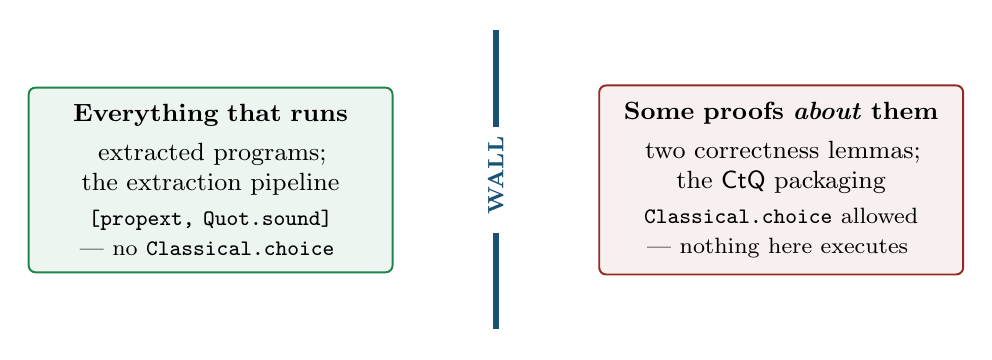
\begin{tikzpicture}
  \node[boxg,text width=42mm,align=center](l){\textbf{Everything that runs}\\[3pt]
    extracted programs;\\ the extraction pipeline\\[3pt]
    \footnotesize \code{[propext, Quot.sound]}\\ --- no \code{Classical.choice}};
  \node[boxb,text width=42mm,align=center,right=26mm of l](r){\textbf{Some proofs \emph{about} them}\\[3pt]
    two correctness lemmas;\\ the $\CtQ$ packaging\\[3pt]
    \footnotesize \code{Classical.choice} allowed\\ --- nothing here executes};
  \draw[line width=2pt,accent]
    ($(l.north east)!0.5!(r.north west)+(0,7mm)$) --
    ($(l.south east)!0.5!(r.south west)-(0,7mm)$)
    node[midway,fill=white,rotate=90,font=\footnotesize\bfseries,text=accent]{~WALL~};
\end{tikzpicture}
\caption{The constructivity wall. On one side, everything that executes ---
choice-free, resting only on the inert kernel axioms. On the other, some proofs
\emph{about} those programs and one packaging step, which may use choice freely
because nothing there ever runs. The one non-constructive axiom in the whole
development is quarantined on the far side from anything that computes.}
\label{fig:wall}
\end{figure}

A proof needing strictly more than Peano arithmetic --- transfinite induction to
$\epsz$ --- became a program, and the program is \emph{constructive to the last
axiom the machine can name}. The strength went into proving the theorem; none of
it leaked into the thing that runs.

%======================================================================
\section{Act VI --- What the machine forced us to discover}

A proof assistant is usually cast as a checker: you have the argument, it
confirms you made no mistake. That is the smaller half of what happened here.
The larger half is that the machine, by refusing to accept certain things,
\emph{forced} decisions that would never have surfaced on paper --- where a
wave of the hand carries you past exactly the spots where it dug in. Four
episodes; each is a place where the development is shaped the way it is because
the machine would not let it be otherwise.

\subsection*{The level bookkeeping was not designed --- it was extorted}

Act~III's realizers live in a tower of types, and each formula carries a level
saying how high in the tower its realizers sit. The rule turned out to be
sharp:
\begin{keystmt}
Connectives that \emph{consume} a realizer --- implication and ``for all'' ---
cost a level. Connectives that merely \emph{package} realizers --- ``and,''
``or,'' and ``there exists'' --- cost nothing.
\end{keystmt}
On paper one might guess a level discipline and tune it until the proofs go
through. Here there was no room to guess: assign ``there exists'' a level it
should not have, or deny ``for all'' the level it needs, and the realizer types
fail to line up and the type-checker rejects the extractor outright --- not with
a warning, with a hard error at the exact malformed clause. The rule above was
read off the pattern of what the machine accepted and what it refused. The
distinction it encodes --- consuming versus packaging --- is a real conceptual
fault line in realizability, and it was the type-checker that drew it.

\subsection*{The Hydra boundary was provable, not merely felt}

Act~IV ended at the wall where the general Kirby--Paris theorem cannot be stated
in the fragment. On paper that is easy to slide past --- one writes ``for every
strategy\dots'' and reads it as innocent. Inside the machine it is not innocent:
to write it you must produce a term quantifying over functions, and the
fragment's grammar has no such term former. The attempt does not produce a weak
or unprovable statement; it produces \emph{no statement at all}, because it does
not parse. The split between the fragment theorem (one battle) and the
metatheorem (all strategies) is therefore not a matter of taste about where to
stop --- it is forced by a checkable property of the fragment's syntax. The
machine turned ``this feels out of reach'' into ``this is provably
inexpressible.''

\subsection*{The pairing had to be hand-built, or the audit would have failed}

Act~V's clean verdict --- nothing that runs uses \code{Classical.choice} --- was
nearly lost to a detail three layers down. The $\epsz$ ordinals are encoded as
ordinary numbers, and that encoding needs a way to pack two numbers into one:
a pairing function. The proof-assistant library ships one, ready to use. But its
supporting lemmas are, throughout, proved with \code{Classical.choice} --- and
because the transfinite recursor's very \emph{definition} calls the pairing,
that choice would have flowed downstream into $\extract$ and tainted
\emph{every} extracted program (Figure~\ref{fig:pair}). The paper argument
``we encode ordinals as numbers'' hides this completely; \code{\#print axioms},
run on an early prototype, made it glaring --- \code{Classical.choice} appearing
in a program that should have had none, traced back to the borrowed pairing. The
fix was to hand-roll a triangular pairing that the kernel can compute and whose
lemmas are choice-free. A foundational decision, invisible on paper, forced into
the open by the audit the machine made possible.

\begin{figure}[h]
\centering
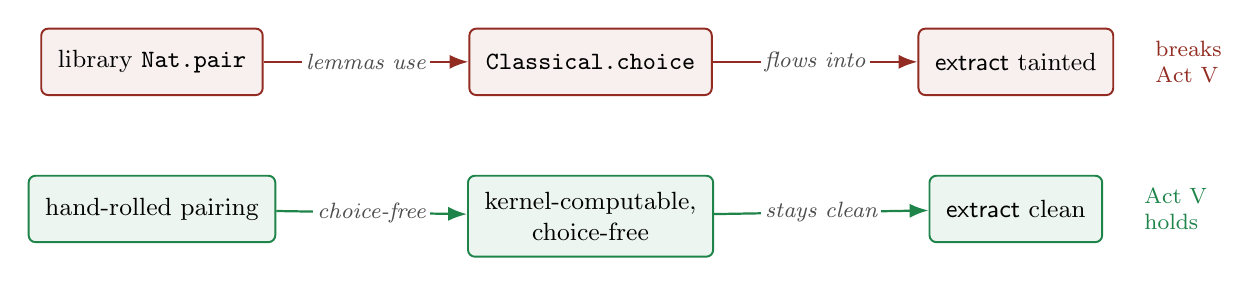
\begin{tikzpicture}[node distance=10mm and 26mm]
  \node[boxb](np){library \code{Nat.pair}};
  \node[boxb,right=of np](cc){\code{Classical.choice}};
  \node[boxb,right=of cc](ex1){$\extract$ tainted};
  \draw[flow,draw=bad](np)--node[elabel]{lemmas use}(cc);
  \draw[flow,draw=bad](cc)--node[elabel]{flows into}(ex1);
  \node[figcap,right=4mm of ex1,text=bad,align=left]{breaks\\ Act~V};
  \node[boxg,below=of np](hp){hand-rolled pairing};
  \node[boxg,below=of cc](cf){kernel-computable,\\ choice-free};
  \node[boxg,below=of ex1](ex2){$\extract$ clean};
  \draw[flow,draw=good](hp)--node[elabel]{choice-free}(cf);
  \draw[flow,draw=good](cf)--node[elabel]{stays clean}(ex2);
  \node[figcap,right=4mm of ex2,text=good,align=left]{Act~V\\ holds};
\end{tikzpicture}
\caption{The discovery the audit forced. Reusing the library's pairing (top)
would have threaded \code{Classical.choice} through the ordinal recursor into
every extracted program. Hand-rolling a choice-free pairing (bottom) keeps the
one non-constructive axiom out of everything that runs. The leak was invisible
on paper and glaring under \code{\#print axioms}.}
\label{fig:pair}
\end{figure}

\subsection*{A verified optimization that changed nothing --- and we kept it}

The transfinite recursor is the development's most expensive machine, so an
obvious improvement suggests itself: \emph{memoize} it --- cache each ordinal's
result so it is not recomputed. This was implemented, proved correct, and wired
in as a drop-in replacement for the plain recursor. Then it was measured, and it
changed \emph{nothing}. The reason is precise and only visible once you look:
producing the recursor's value at an ordinal code is already a constant-time
operation --- it hands back a closure --- so the real cost lives in the
\emph{applications} of that closure, which a table keyed by the ordinal code can
never reach. The verified-but-useless memo path is kept in the development, with
its correctness proof, as the record of a negative result that was
\emph{measured} rather than assumed. On paper an optimization that looks
plausible tends to get written up as a win; here the profiler said otherwise, and
honesty about the null result was cheaper than the illusion of a speedup.

\subsection*{The descent was demoted from assumption to theorem}

The engine of Goodstein and the Hydra is one fact: each step strictly lowers the
ordinal. In an early version that fact was simply \emph{assumed} --- imported as
an axiom schema and used. That is a real dependency, and the machine records it:
an assumed descent appears on the \code{\#print axioms} list, in plain sight,
for anyone to see how much is being taken on faith. The development later
\emph{earned} it back, deriving the descent from three small schemas, each about
a single symbol in relation to a single ordinal operation, none mentioning
Goodstein or the Hydra at all. The gain is not that the proof got shorter --- it
is that the ledger of assumptions got smaller, and the machine is what keeps that
ledger honest. What you assume is visible; reducing it is progress you can point
to, not a matter of narrative.

%======================================================================
\section{Act VII --- The thesis}

Set the examples back-to-back --- Hanoi, Pascal, Fibonacci, Euclid, Sperner,
Goodstein, the Hydra --- and the natural summary is ``look, one pipeline turns
proofs into programs.'' But that pipeline is old news: that a constructive proof
carries computational content is the content of realizability and of the
Curry--Howard correspondence~\citep{howard1980}, both decades established. The reader was told as
much in Act~I, and being shown a known correspondence at work is not, by itself,
a surprise --- though Figure~\ref{fig:curry-howard} makes it unusually concrete,
reading the extracted program back onto the proof of the hardest theorem here.

\begin{figure}[h]
\centering
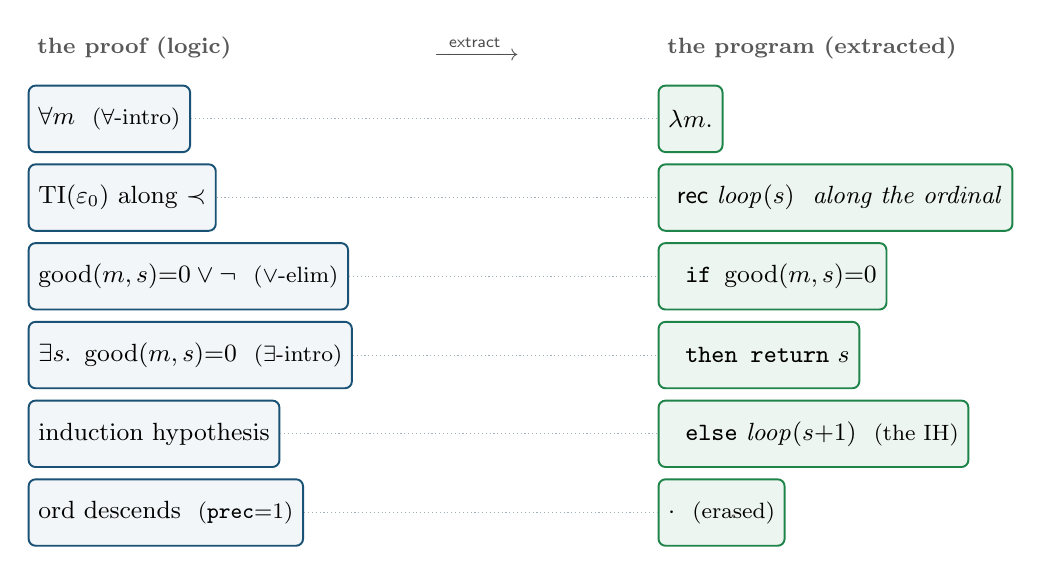
\begin{tikzpicture}[
   L/.style={box,anchor=west,align=left,inner sep=3.5pt,font=\small},
   R/.style={boxg,anchor=west,align=left,inner sep=3.5pt,font=\small}]
  \node[figcap,anchor=west,font=\footnotesize\bfseries] at (0,9mm){the proof (logic)};
  \node[figcap,anchor=west,font=\footnotesize\bfseries] at (80mm,9mm){the program (extracted)};
  \node[elabel] at (57mm,9mm){$\xrightarrow{\ \extract\ }$};
  \node[L,anchor=west] (l1) at (0,  0mm){$\forall m$ \ \footnotesize($\forall$-intro)};
  \node[L,anchor=west] (l2) at (0,-10mm){$\mathrm{TI}(\epsz)$ along $\prec$};
  \node[L,anchor=west] (l3) at (0,-20mm){$\good(m,s){=}0 \lor \neg$ \ \footnotesize($\lor$-elim)};
  \node[L,anchor=west] (l4) at (0,-30mm){$\exists s.\ \good(m,s){=}0$ \ \footnotesize($\exists$-intro)};
  \node[L,anchor=west] (l5) at (0,-40mm){induction hypothesis};
  \node[L,anchor=west] (l6) at (0,-50mm){$\mathrm{ord}$ descends \ \footnotesize($\code{prec}{=}1$)};
  \node[R,anchor=west] (r1) at (80mm,  0mm){$\lambda m.$};
  \node[R,anchor=west] (r2) at (80mm,-10mm){$\ \mathsf{rec}\ \mathit{loop}(s)$ \emph{ along the ordinal}};
  \node[R,anchor=west] (r3) at (80mm,-20mm){$\ \ \code{if}\ \good(m,s){=}0$};
  \node[R,anchor=west] (r4) at (80mm,-30mm){$\ \ \code{then return}\ s$};
  \node[R,anchor=west] (r5) at (80mm,-40mm){$\ \ \code{else}\ \mathit{loop}(s{+}1)$ \ \footnotesize(the IH)};
  \node[R,anchor=west] (r6) at (80mm,-50mm){$\cdot$ \ \footnotesize(erased)};
  \foreach \i in {1,2,3,4,5,6} \draw[densely dotted,rulec] (l\i.east) -- (r\i.west);
\end{tikzpicture}
\caption{\textbf{The extraction map on the hardest theorem.} Modified
realizability is Curry--Howard with the map made explicit: $\extract$ sends each
proof rule (left) to one program operation (right). A witness supplied by hand
extracts to a constant --- $\exists s.\ \good(3,s){=}0$, proved by $\code{exI}\
5$, gives \code{return}$\ \langle 5,\cdot\rangle$ --- while a witness produced by
transfinite induction extracts to a recursion, the shape of the induction
becoming the shape of the recursion. The induction hypothesis \emph{is} the
recursive call; the ordinal descent, carrying no runtime content, is erased. The
same object is a proof that every Goodstein sequence terminates and a program
that computes when. What is old is the correspondence; what is new is that this
one fixed apparatus reaches $\mathrm{TI}(\epsz)$ with nothing added.}
\label{fig:curry-howard}
\end{figure}

The surprise is the \emph{range reached with so little}. One signature of
twenty-one symbols. One extractor, with one small combinator per inference rule.
One soundness proof, one case per rule. One continuity invariant, closed under
the same handful of combinators. That fixed, modest apparatus --- never enlarged
across the whole tour --- was enough to reach a structured puzzle solution, a
decision procedure that draws the Sierpi\'nski triangle, a strengthened-invariant
iterator, a greatest-common-divisor calculator, a discrete intermediate-value
search, and two theorems --- Goodstein and Kirby--Paris --- that genuinely need
transfinite induction to $\epsz$, more than ordinary arithmetic can prove. Wildly
different mathematics; the same few moving parts.

And the whole way down, the machine kept the accounting honest --- not as a
formality but as the thing that made the strongest claim sayable at all. The
constructivity verdict of Act~V is not an aspiration one hopes holds up under
scrutiny; it is a fact the kernel will reprint on demand, for every program in
the development: everything that runs rests on two inert axioms and nothing
classical. A proof that needs more than Peano arithmetic became a program that
needs less than a whiff of choice --- and we know it needs less because the
machine, asked directly, said so.

That is how a proof becomes a program: not by a grand mechanism, but by a small
one applied with discipline, and checked by something that cannot be talked past.

\bibliographystyle{plainnat}
\bibliography{refs}

\end{document}
